\documentclass[compress]{beamer}

\usetheme{Luebeck}
\usepackage[utf8]{inputenc}
\usepackage{subfig}
\usepackage{utopia} %font utopia imported
\usepackage{arabtex}
\usepackage{utf8}
\setcode{utf8}
\usepackage{amsmath}
\usepackage{amssymb}
\usepackage{amsthm}

\usefonttheme{professionalfonts} % using non standard fonts for beamer
\definecolor{foo}{RGB}{106,141,143}
\usecolortheme[named=foo]{structure}
\setbeamercolor{subsection in head/foot}{bg=foo!80!black}
% This block of code defines the information to appear in the
% title page

\title[ASIC Physical Design] %optional
{FloorPlanning}

\subtitle{How to Plan your own chip}

\author[Ahmed Abdelazeem] % (optional)
{Ahmed Abdelazeem}
%{A.~B.~Arthur\inst{1} \and J.~Doe\inst{2}}

\institute[ZU] % (optional)
{
	Faculty of Engineering\\
	Zagazig University
}
%{
	%	\inst{1}%
	%	Faculty of Engineering\\
	%	Zagazig University
	%	\and
	%	\inst{2}%
	%	Faculty of Chemistry\\
	%	Very Famous University
	%}

\date[ZU 2023] % (optional)
{RTL2GDSII Flow, February 2022}

%\logo{
\includegraphics[height=1.5cm]{lion-logo.png}}

%End of title page configuration block
%------------------------------------------------------------

%------------------------------------------------------------
%The next block of commands puts the table of contents at the
%beginning of each section and highlights the current section:
\setcounter{tocdepth}{1} %%%
\AtBeginSection[]
{
	\begin{frame}
		\frametitle{Table of Contents}
		\tableofcontents[currentsection]
	\end{frame}
}
%------------------------------------------------------------


\begin{document}
	
	%The next statement creates the title page.
	\frame{\titlepage}
	
	
	%---------------------------------------------------------
	%This block of code is for the table of contents after
	%the title page
	\begin{frame}
		\frametitle{Table of Contents}
		\tableofcontents
	\end{frame}
	%---------------------------------------------------------
	%--------------------------------------------------
	\section[Intro]{Introduction}
	\subsection[Overall]{Overall Design Flow}
	\begin{frame}
		\frametitle{Overall Design Flow}
		
		\begin{center}
			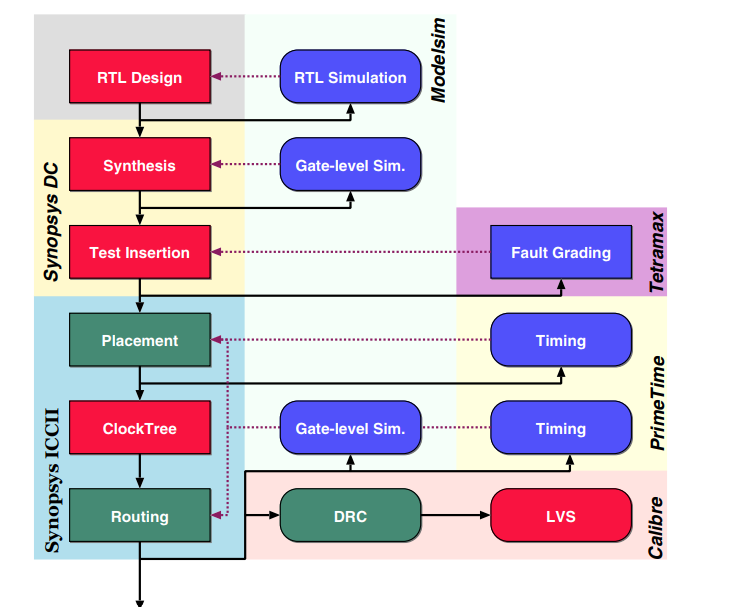
\includegraphics[width=0.8\textwidth]{over}
		\end{center}
	\end{frame}	
	%--------------------------------------------------
	\begin{frame}
		\frametitle{The Big Picture...}
		b
	\end{frame}
	%---------------------------------------------------
	\subsection[setup]{Data Setup}
		\begin{frame}
		\frametitle{Data Setup}
		\begin{center}
			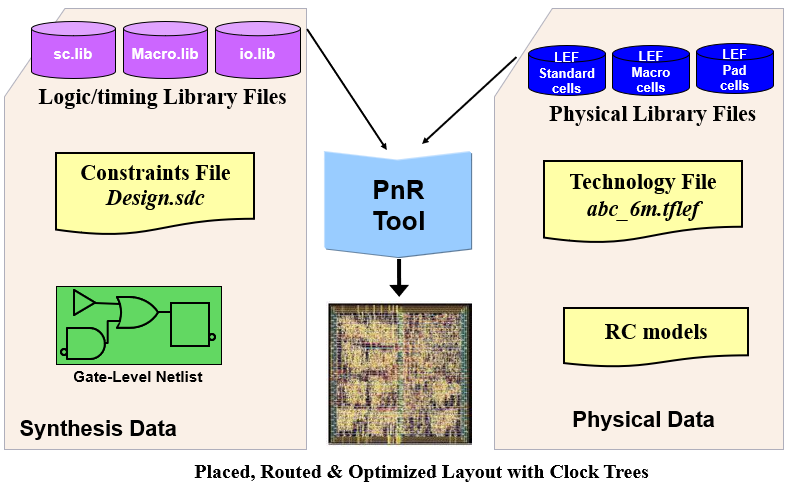
\includegraphics[width=\textwidth]{Datasetup}
		\end{center}
	\end{frame}
\begin{frame}
	\frametitle{Logical Libraries}
		\begin{columns}	
			\column{0.9\textwidth}
			\begin{itemize}
				\item \textbf{Provide} \textcolor{blue}{\textbf{timing}} \textbf{and} \textcolor{blue}{\textbf{functionality}} \textbf{information for all
				standard cells (and, or, flipflop, ...)}
				\item \textbf{Provide} \textcolor{blue}{\textbf{timing}} \textbf{information for hard macros(IP, ROM, RAM, ...)}
				\item \textbf{Define drive/load design rules:}
					\begin{itemize}
						\item \textcolor{red}{Max fanout}
						\item \textcolor{red}{Max transition}
						\item \textcolor{red}{Max/Min capacitance}
					\end{itemize}
			\item \textbf{Are usually the same ones used by Syntheis during synthesis}
			\end{itemize}
			\column{0.2\textwidth}
			\begin{center}
				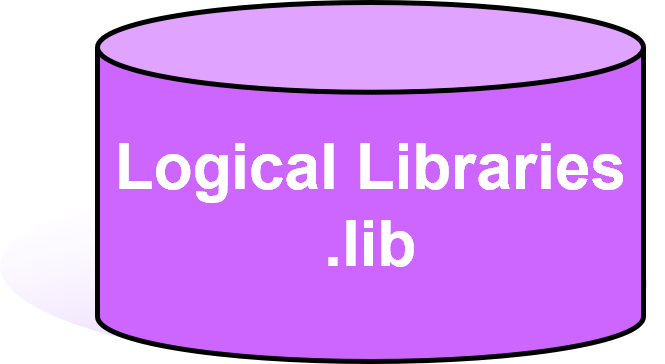
\includegraphics[width=0.9 \textwidth]{lib}
			\end{center}
		\end{columns}
\end{frame}
\begin{frame}
	\frametitle{Timing Constraints}
	\begin{itemize}
		\item “Timing Constraints” are required to communicate the design’s timing intentions to PnR Tool
		\item They should be the same ones used for synthesis with Synthesis Tool (preferably SDC)
	\end{itemize}
	\begin{center}
		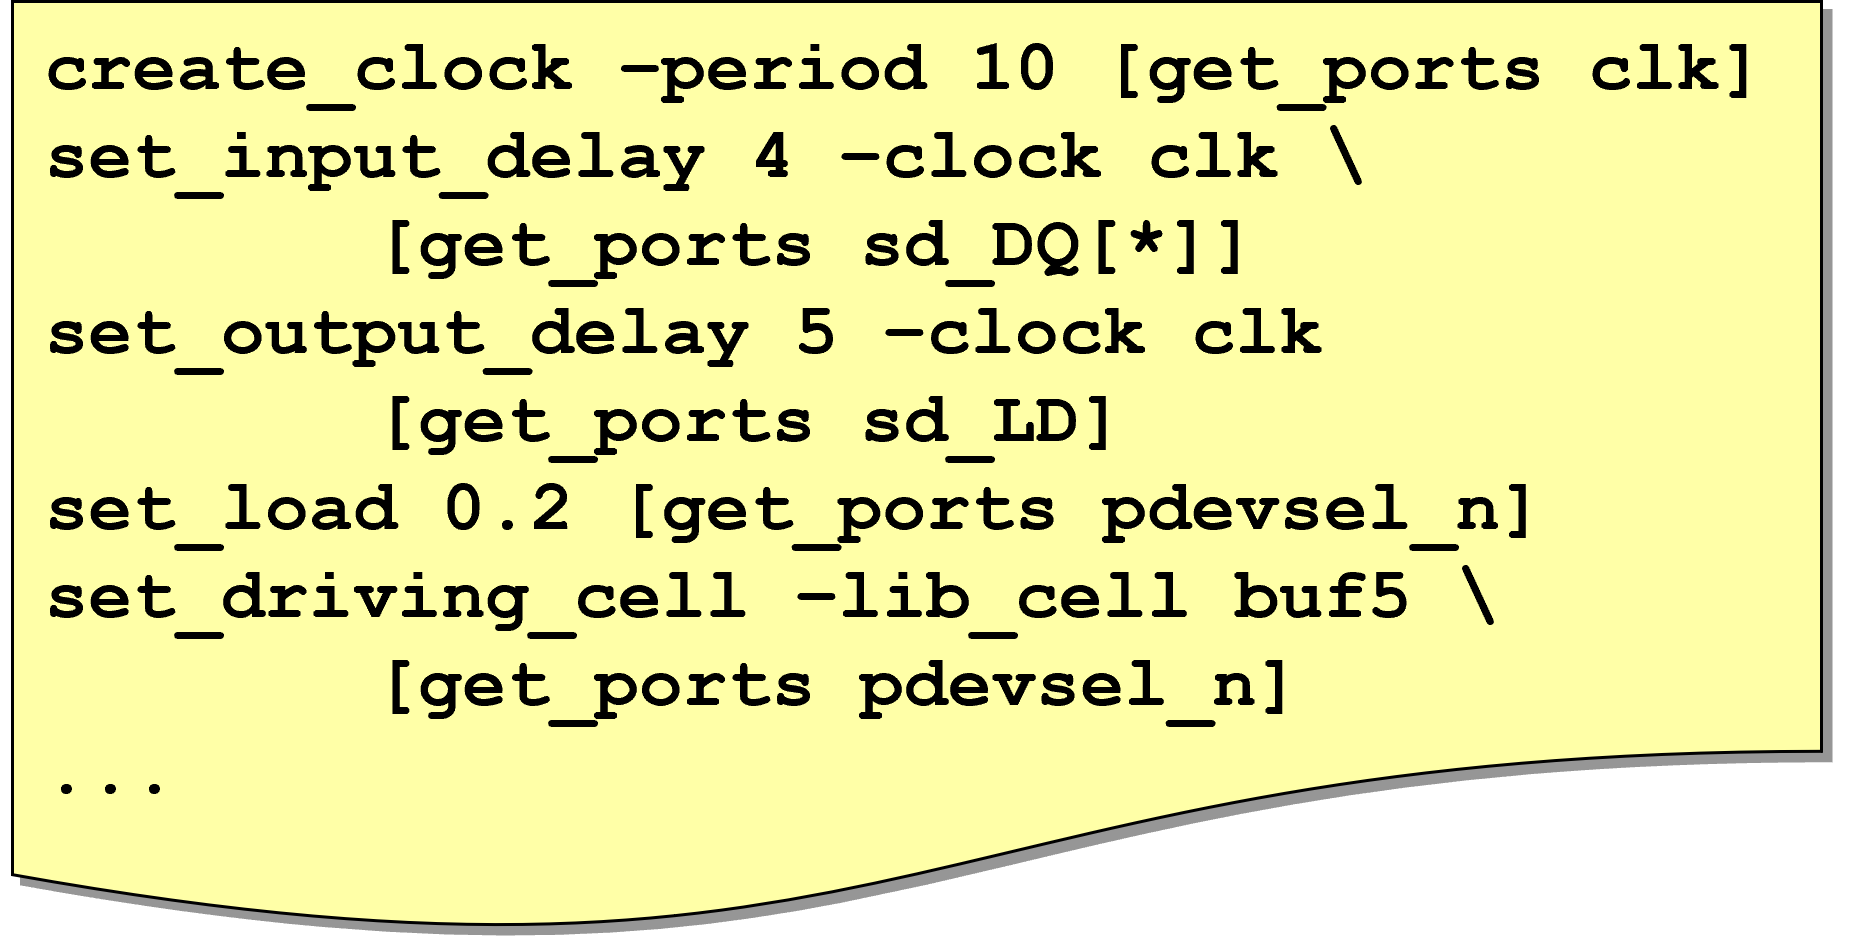
\includegraphics[width=0.8\textwidth]{SDC}
	\end{center}
\end{frame}	
\begin{frame}
	\frametitle{Physical Libraries}
	
		\begin{columns}	
		
			\column{0.7\textwidth}
				\begin{center}
				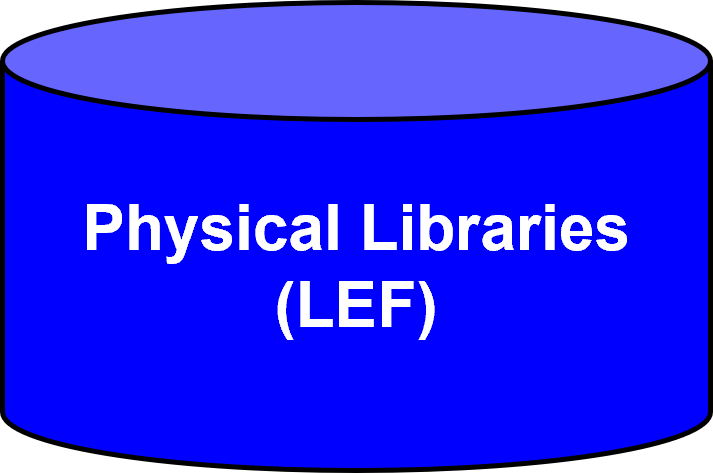
\includegraphics[width=0.3\textwidth]{LEF_1}
			\end{center}
			\begin{itemize}
				\item \textbf{Contain physical information
				of standard, macro and pad
				cells, necessary for placement
				and routing}
				\item \textbf{Define placement unit tile}
				\begin{itemize}
					\item Height of placement rows
					\item Minimum width resolution
					\item Preferred routing directions
					\item Pitch of routing tracks
				\end{itemize}
				
			\end{itemize}
			\column{0.5\textwidth}
			\begin{center}
				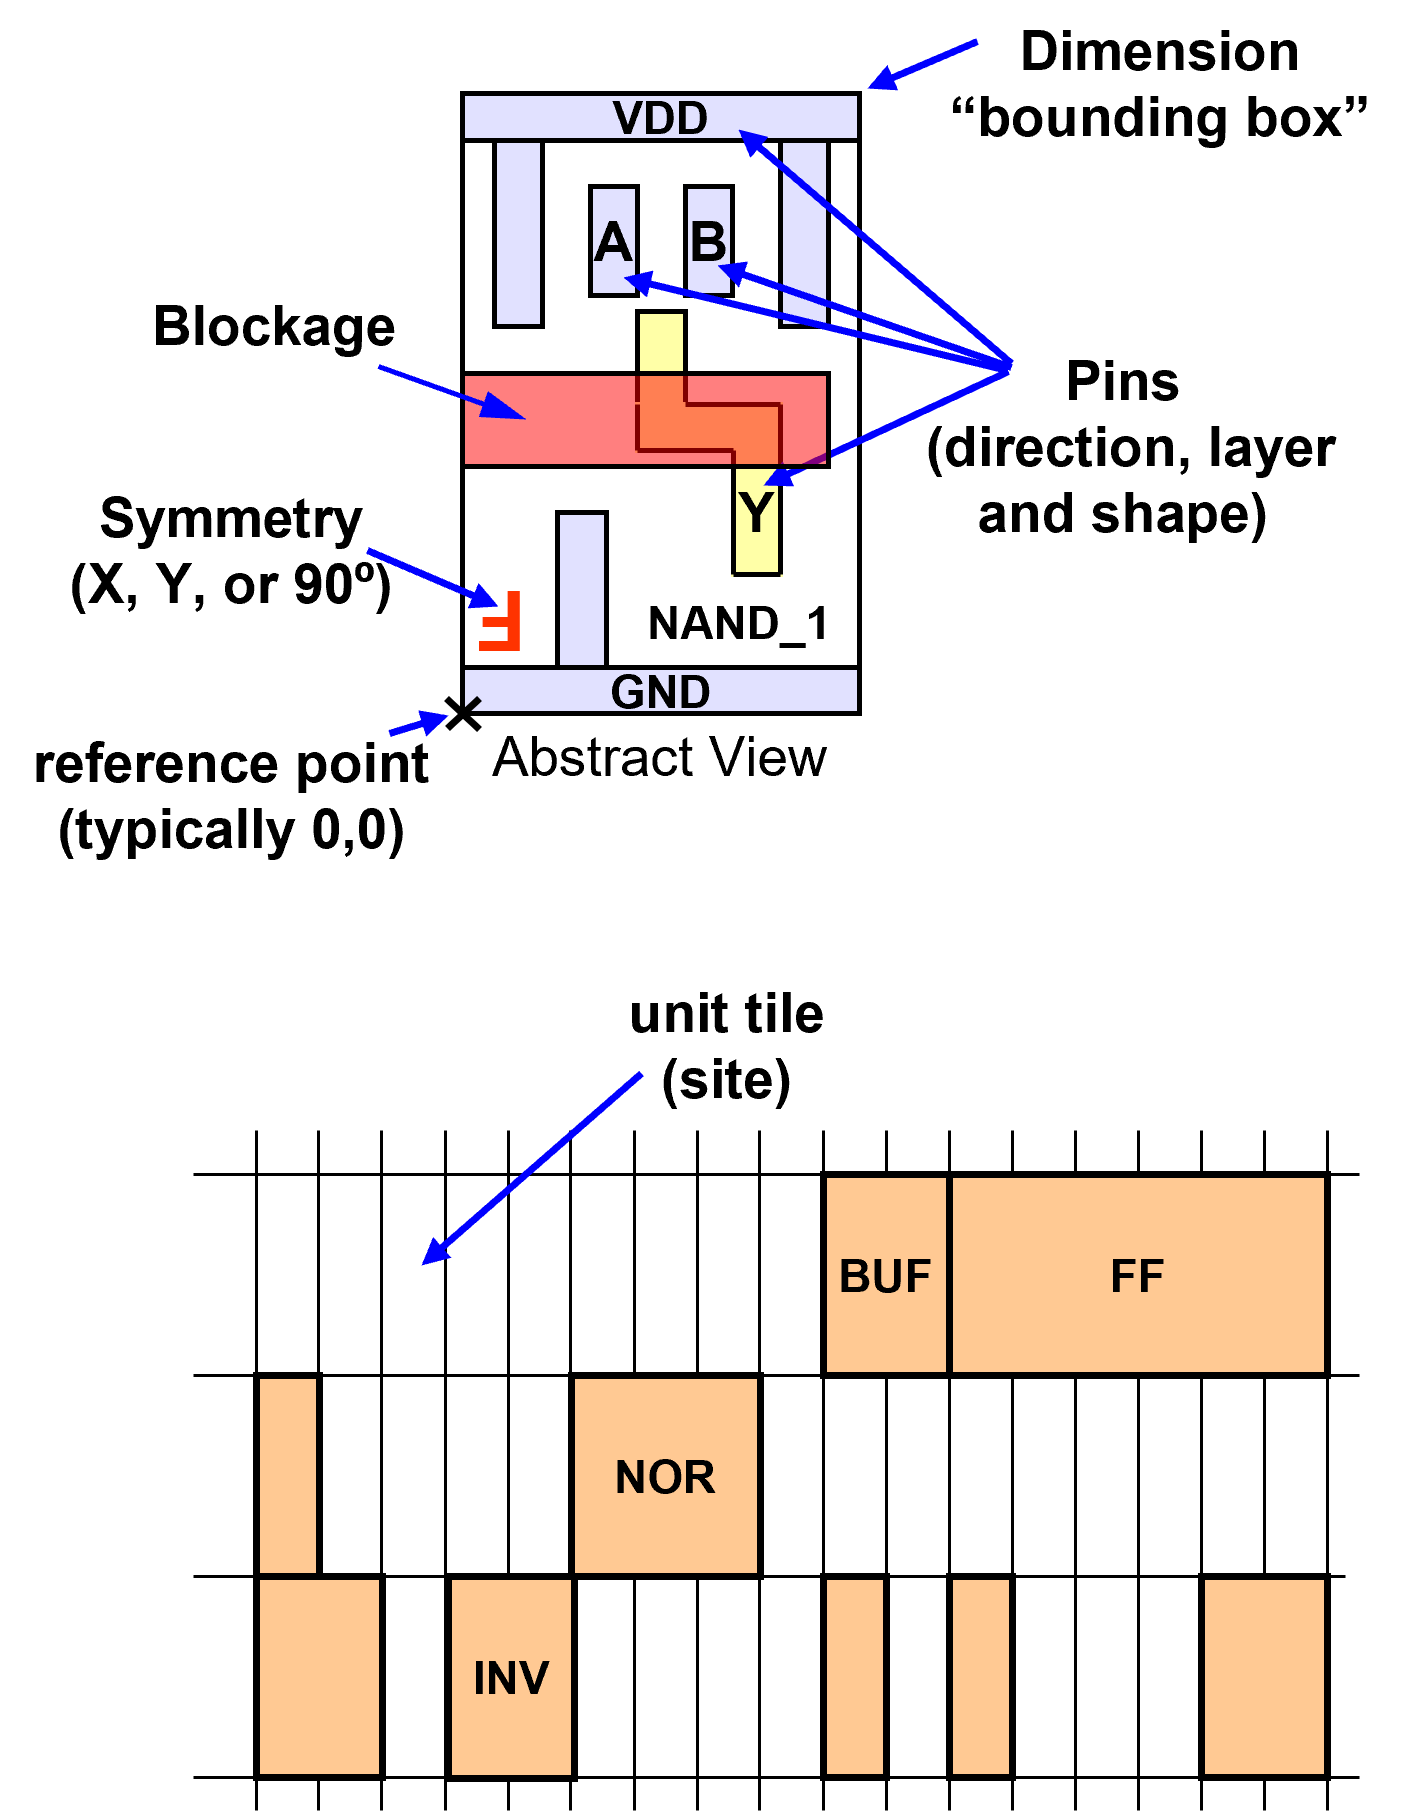
\includegraphics[width=0.8 \textwidth]{LEF}
			\end{center}
		\end{columns}
\end{frame}

\begin{frame}
	\frametitle{Technology File (.tflef file)}
		\begin{itemize}
			\item \textbf{Tech File is unique to each technology}
			\item \textbf{Contains metal layer technology parameters: }
			\begin{itemize}
				\item Number and name designations for each layer/via
				\item Dielectric constant for technology
				\item Physical and electrical characteristics of each layer/via
				\item Design rules for each layer/Via (Minimum wire widths and wire-to-wire spacing, etc.)
				\item Units and precision for electrical units
				\item Colors and patterns of layers for display
				\item ....
			\end{itemize}
		\end{itemize}
\end{frame}

\begin{frame}
	\frametitle{Example of a Technology File }
	\begin{center}
		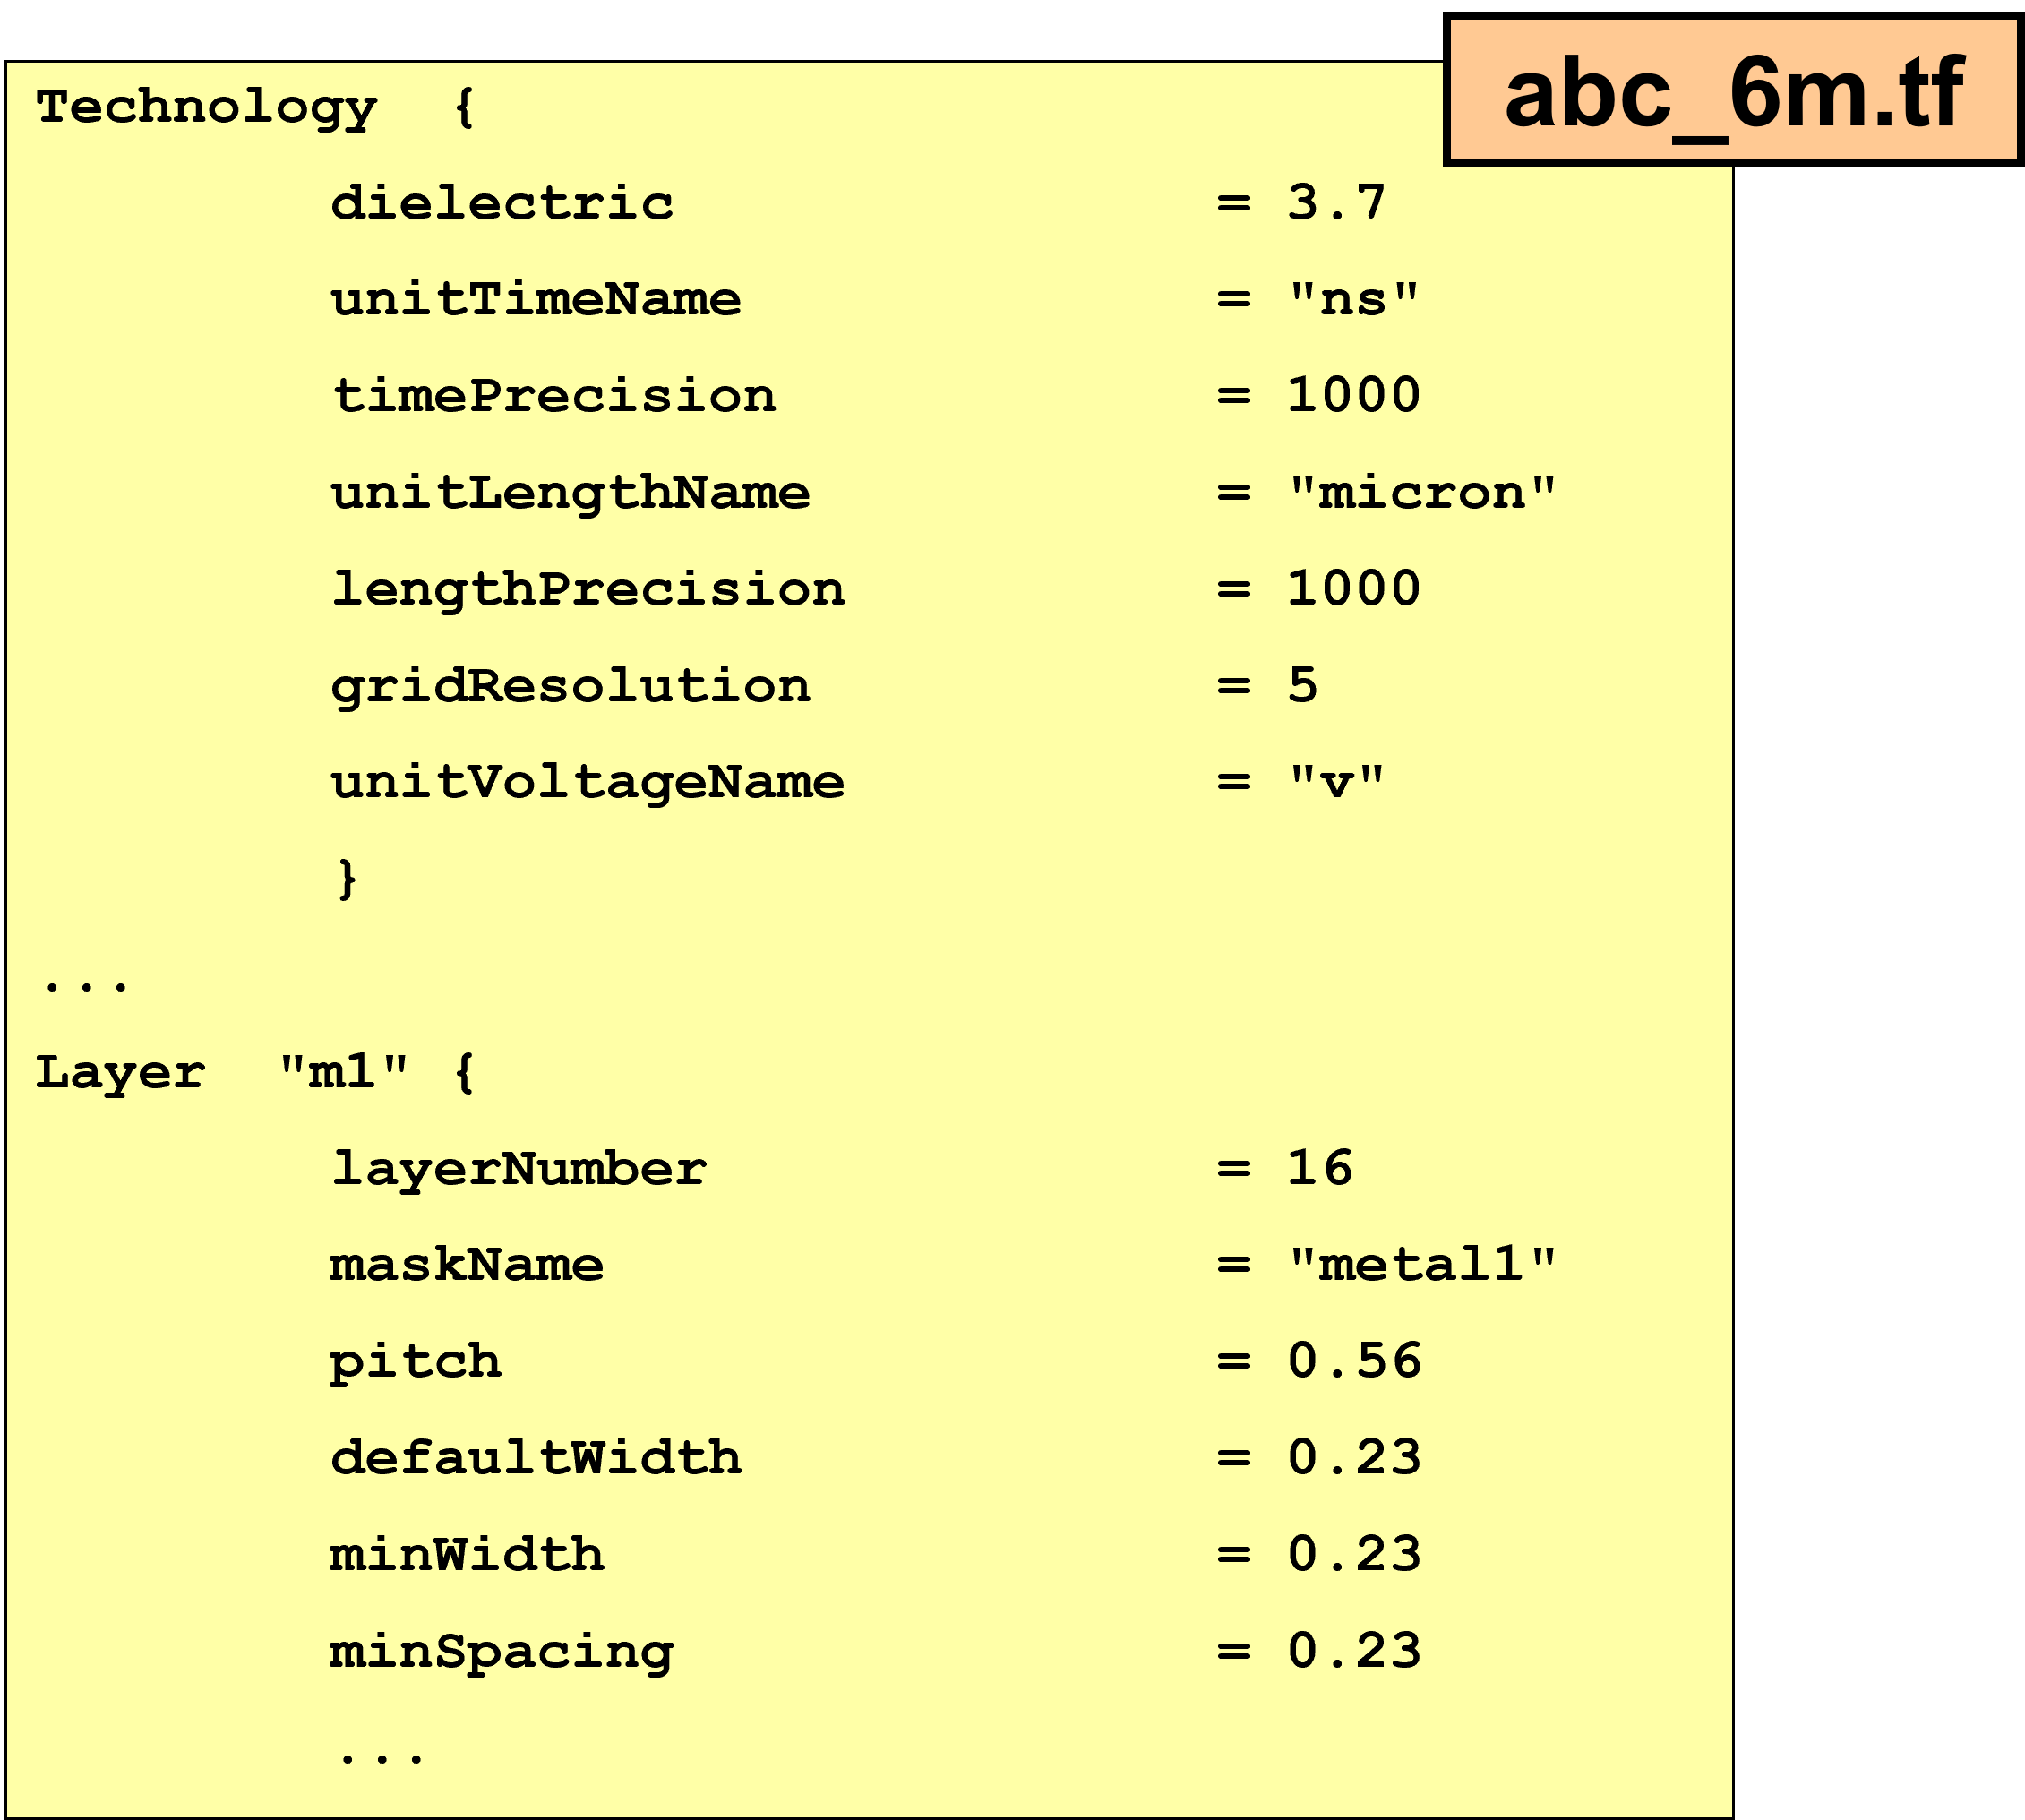
\includegraphics[width=0.7\textwidth]{TF}
	\end{center}
\end{frame}

\begin{frame}
	\frametitle{Timing is Based on Cell and Net Delays}
	\begin{center}
		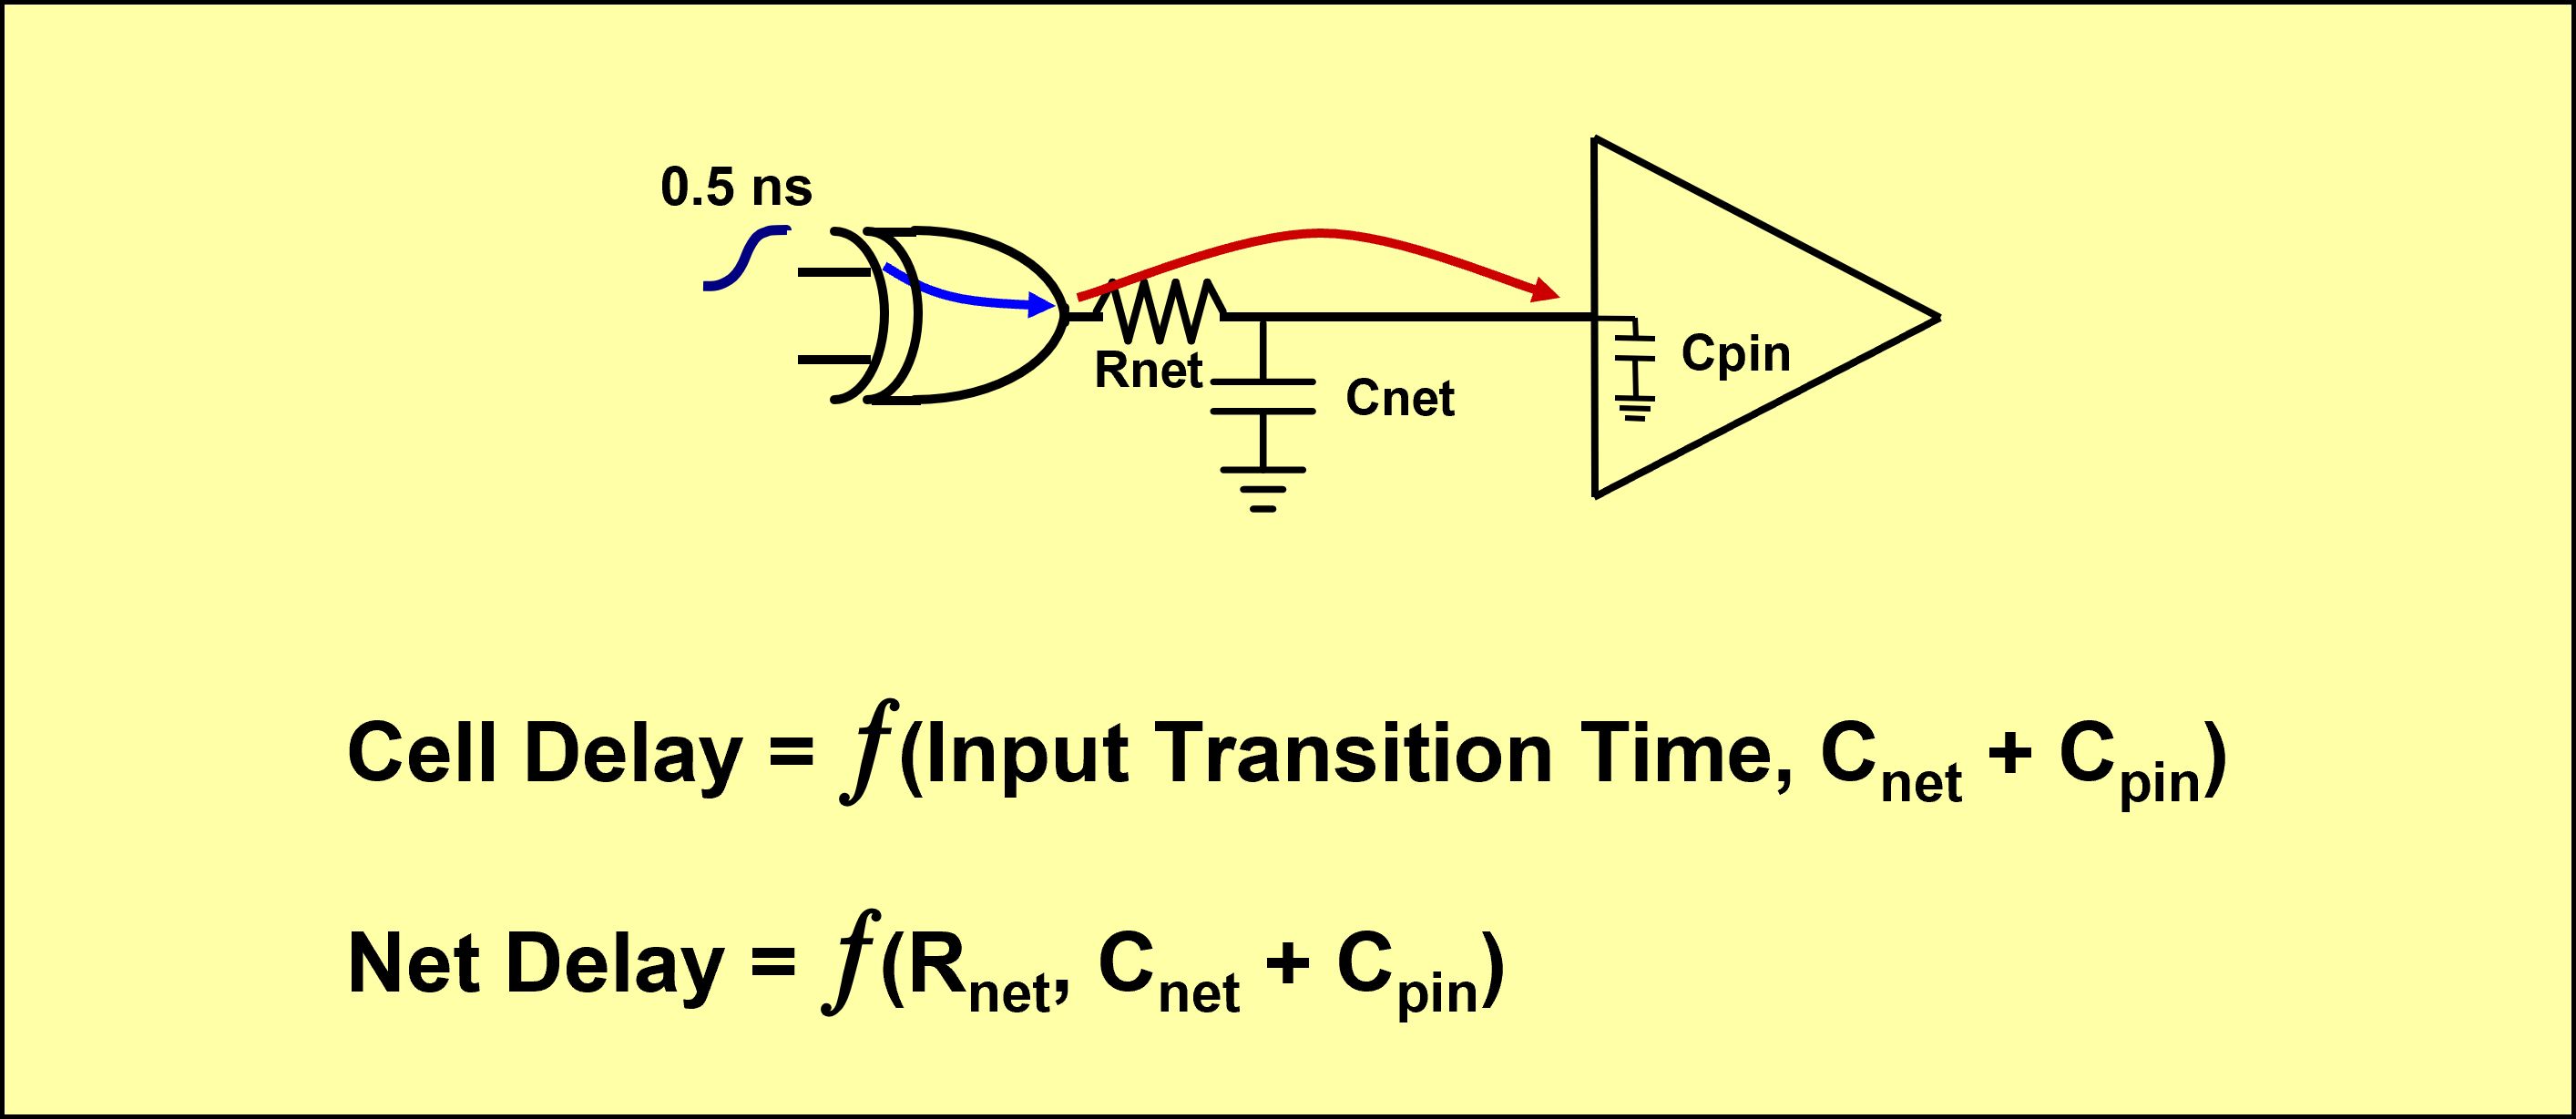
\includegraphics[width=0.6\textwidth]{Time}
	\end{center}
	\begin{itemize}
		\item PnR tool calculates delay for every cell and every net
		\item To calculate delays, tool needs to know each net’s parasitic Rs and Cs
	\end{itemize}
\end{frame}
\begin{frame}
	\frametitle{RC Models}
	\begin{columns}	
		\column{0.7\textwidth}
		\begin{itemize}
			\item \textbf{Tool calculates C and R using the net geometry and the TLU+ look-up tables
			}
			\item \textbf{UDSM process effects modeled}
		\end{itemize}
		\begin{center}
			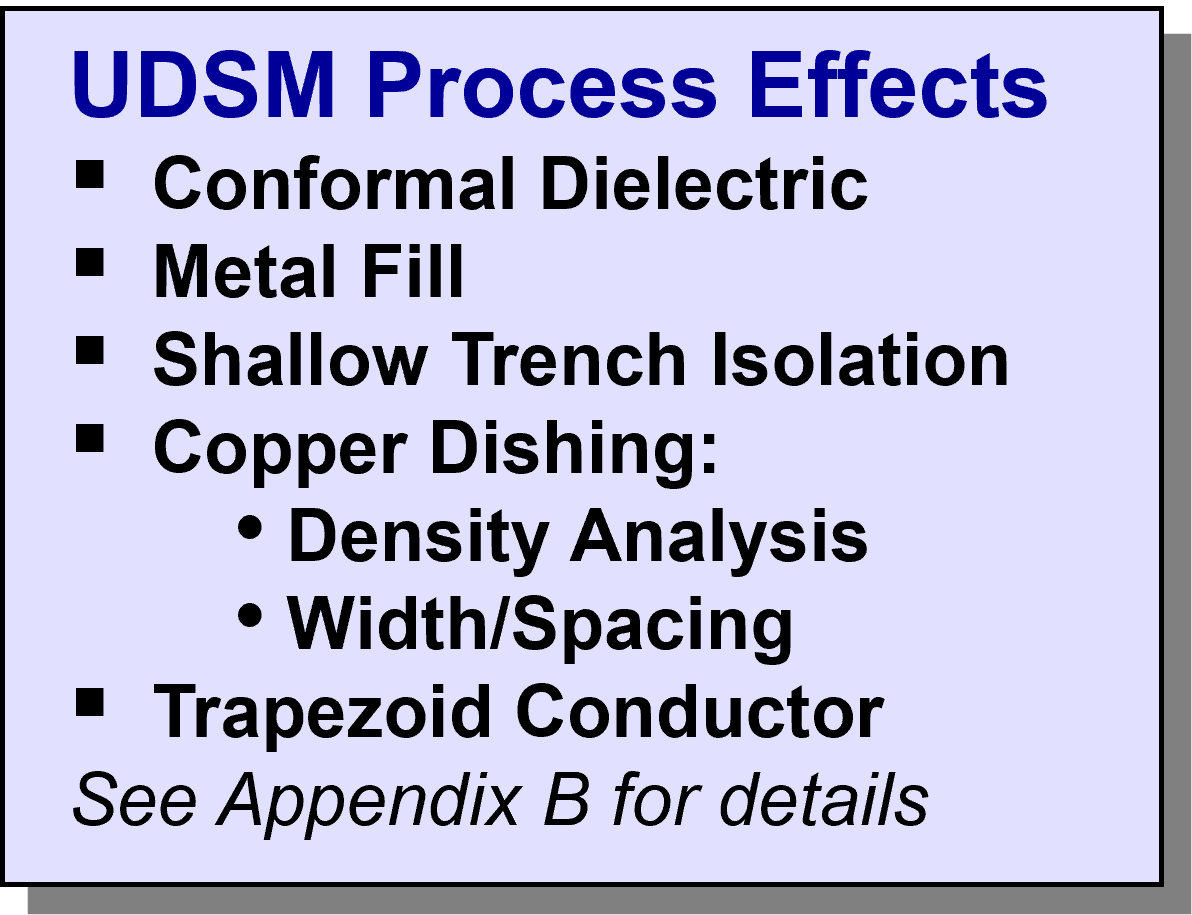
\includegraphics[width=0.6\textwidth]{UDSM}
		\end{center}
		\column{0.5\textwidth}
		\begin{center}
			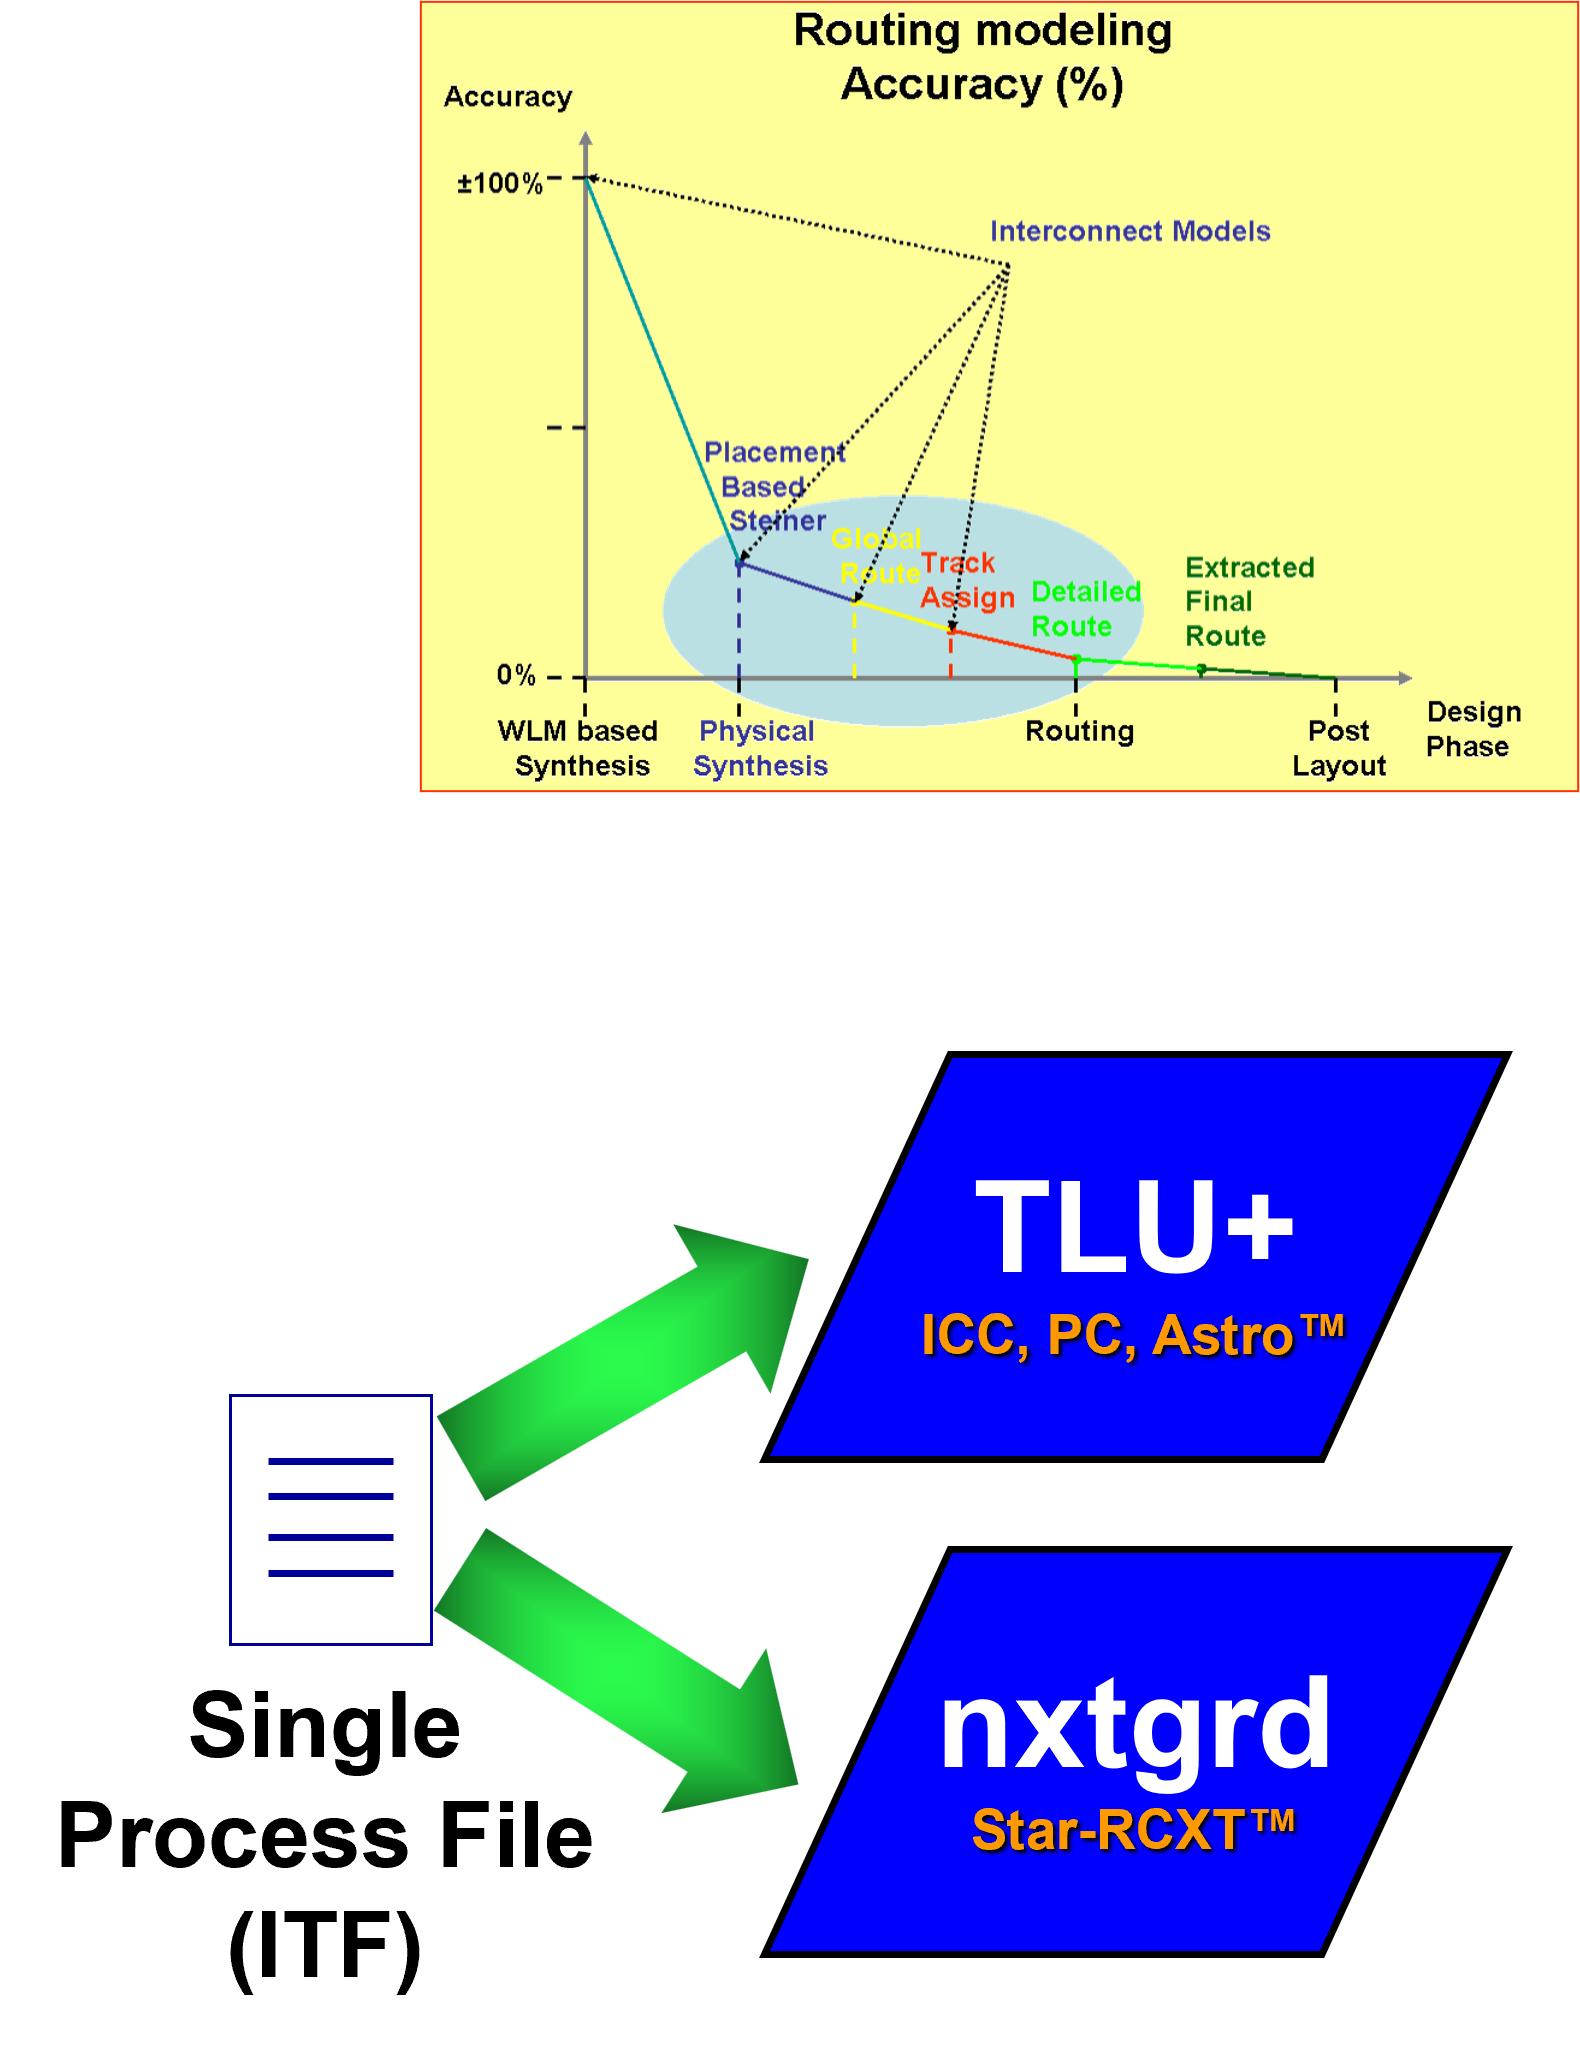
\includegraphics[width=0.8 \textwidth]{TLU}
		\end{center}
	\end{columns}
\end{frame}
\begin{frame}
	\frametitle{Mapping file}
	\textbf{The Mapping File maps the .tf (lef technology file) layer/via names to Star-RCXT .itf layer/via names.}
	
	\begin{center}
		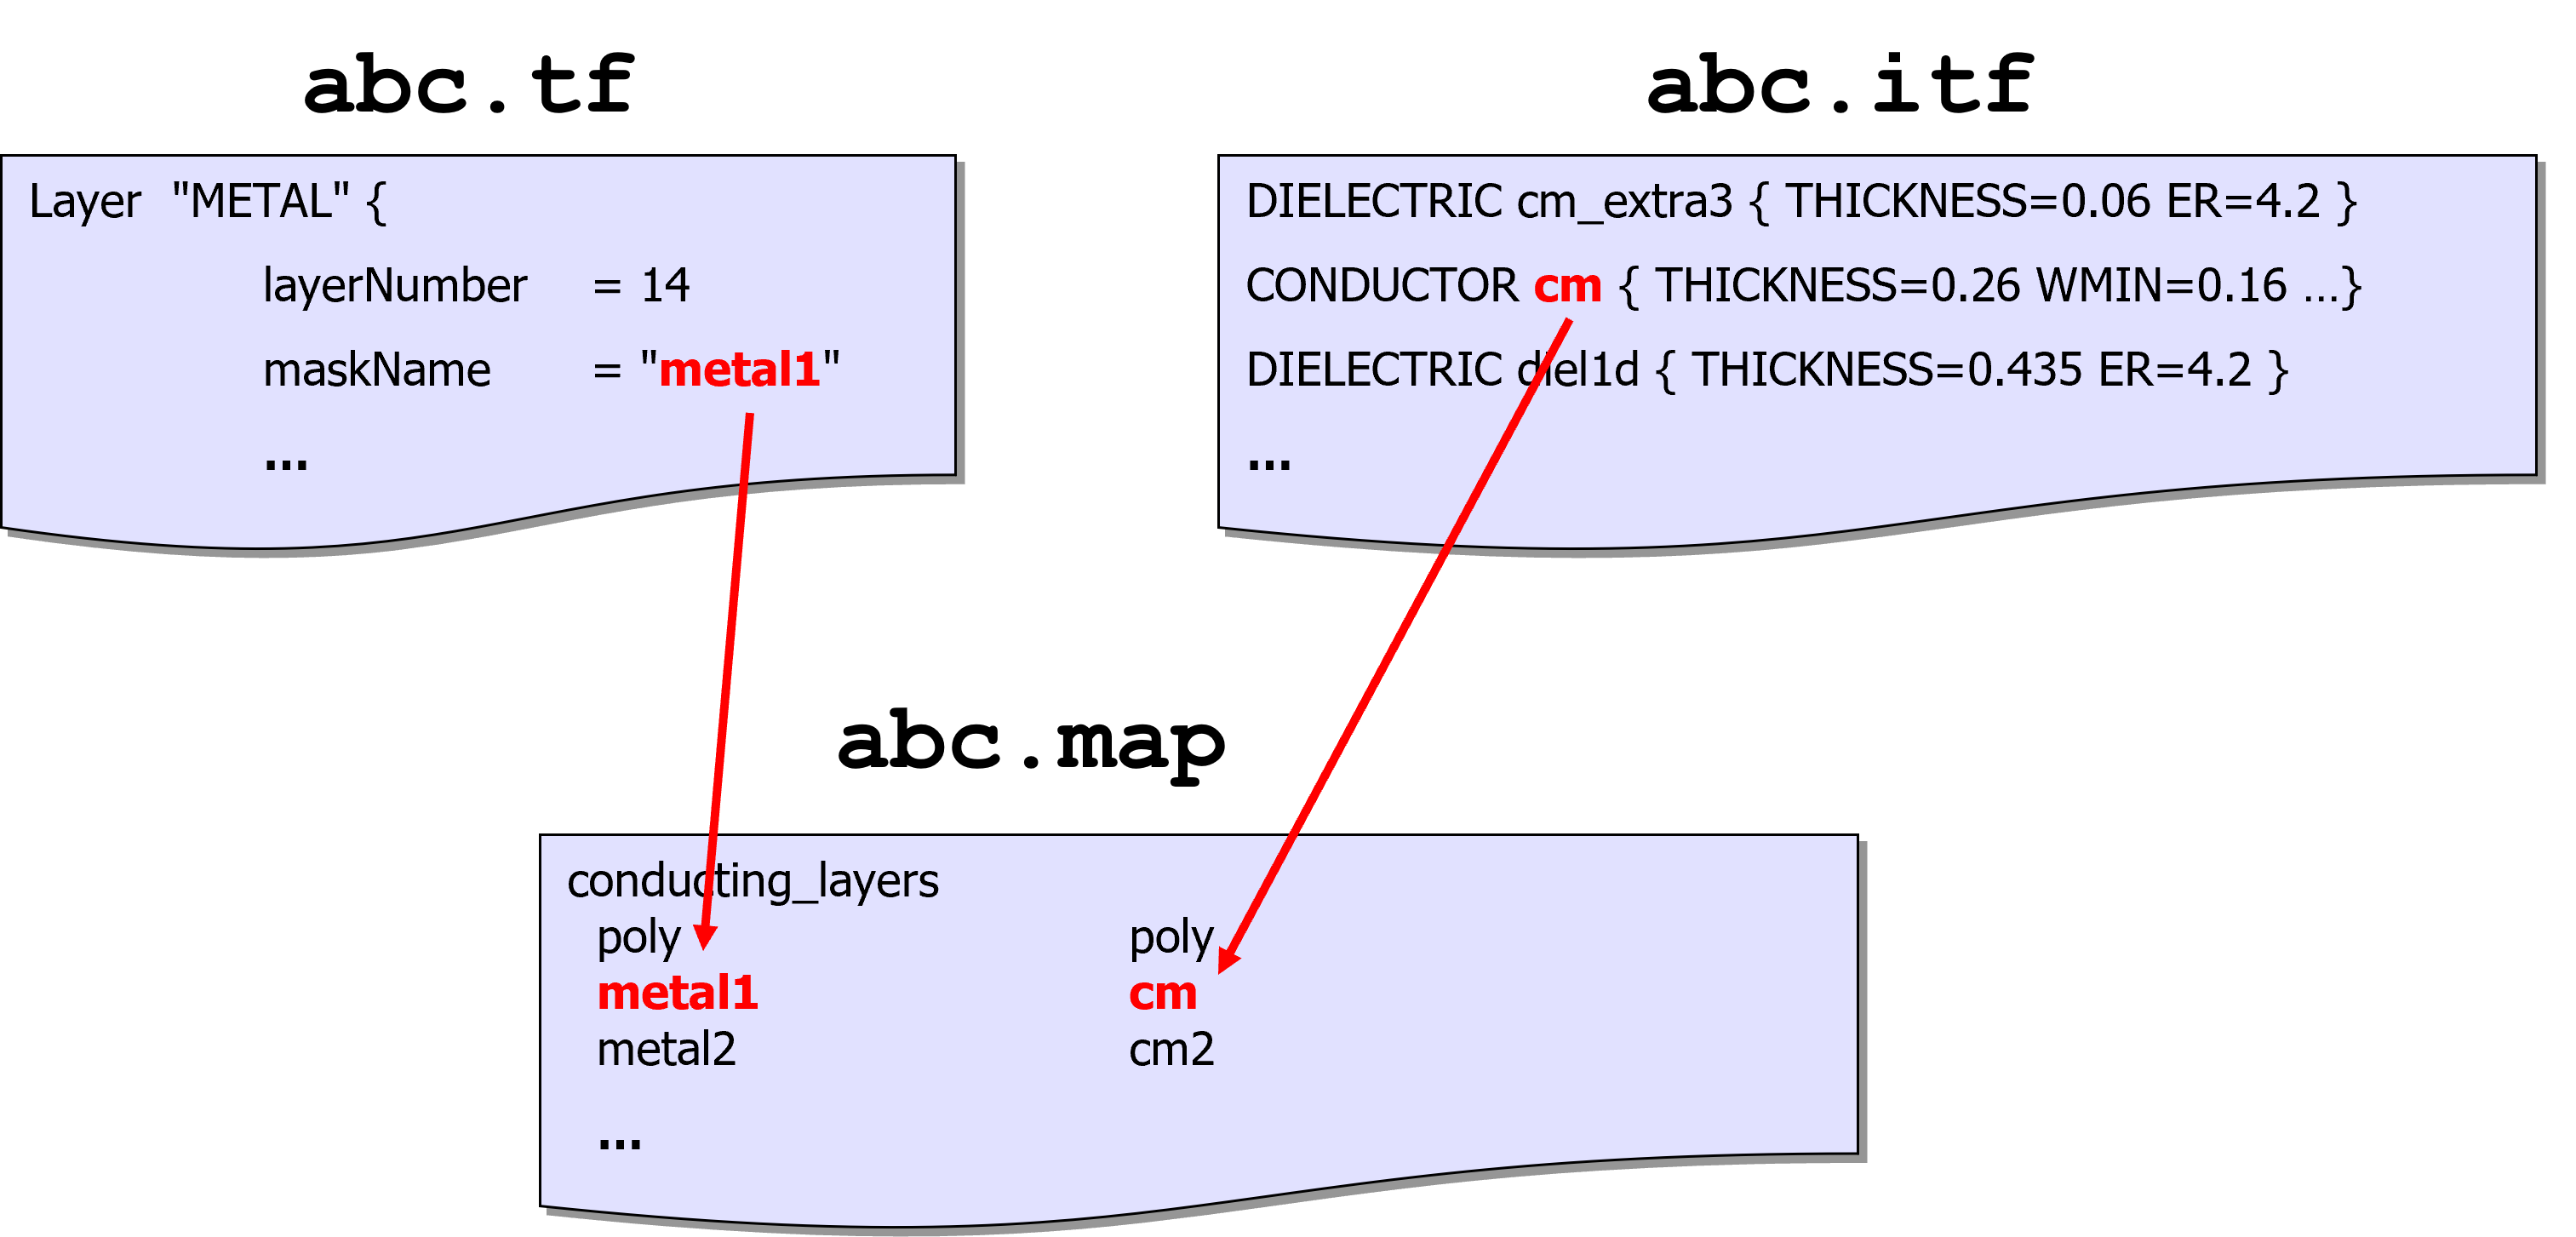
\includegraphics[width=\textwidth]{MAP}
	\end{center}
\end{frame}

\begin{frame}
	\frametitle{Calculating Cell and Net Delay}
	\begin{itemize}
		\item \textbf{Now that R and C are known from TLU+, the delays can be calculated}
		\item\textbf{ For Cell Delays, only} $\textbf{C}_{\textbf{total}}$ / $\textbf{C}_{\textbf{eff}}$ \textbf{is needed}
	\end{itemize}
		\begin{center}
			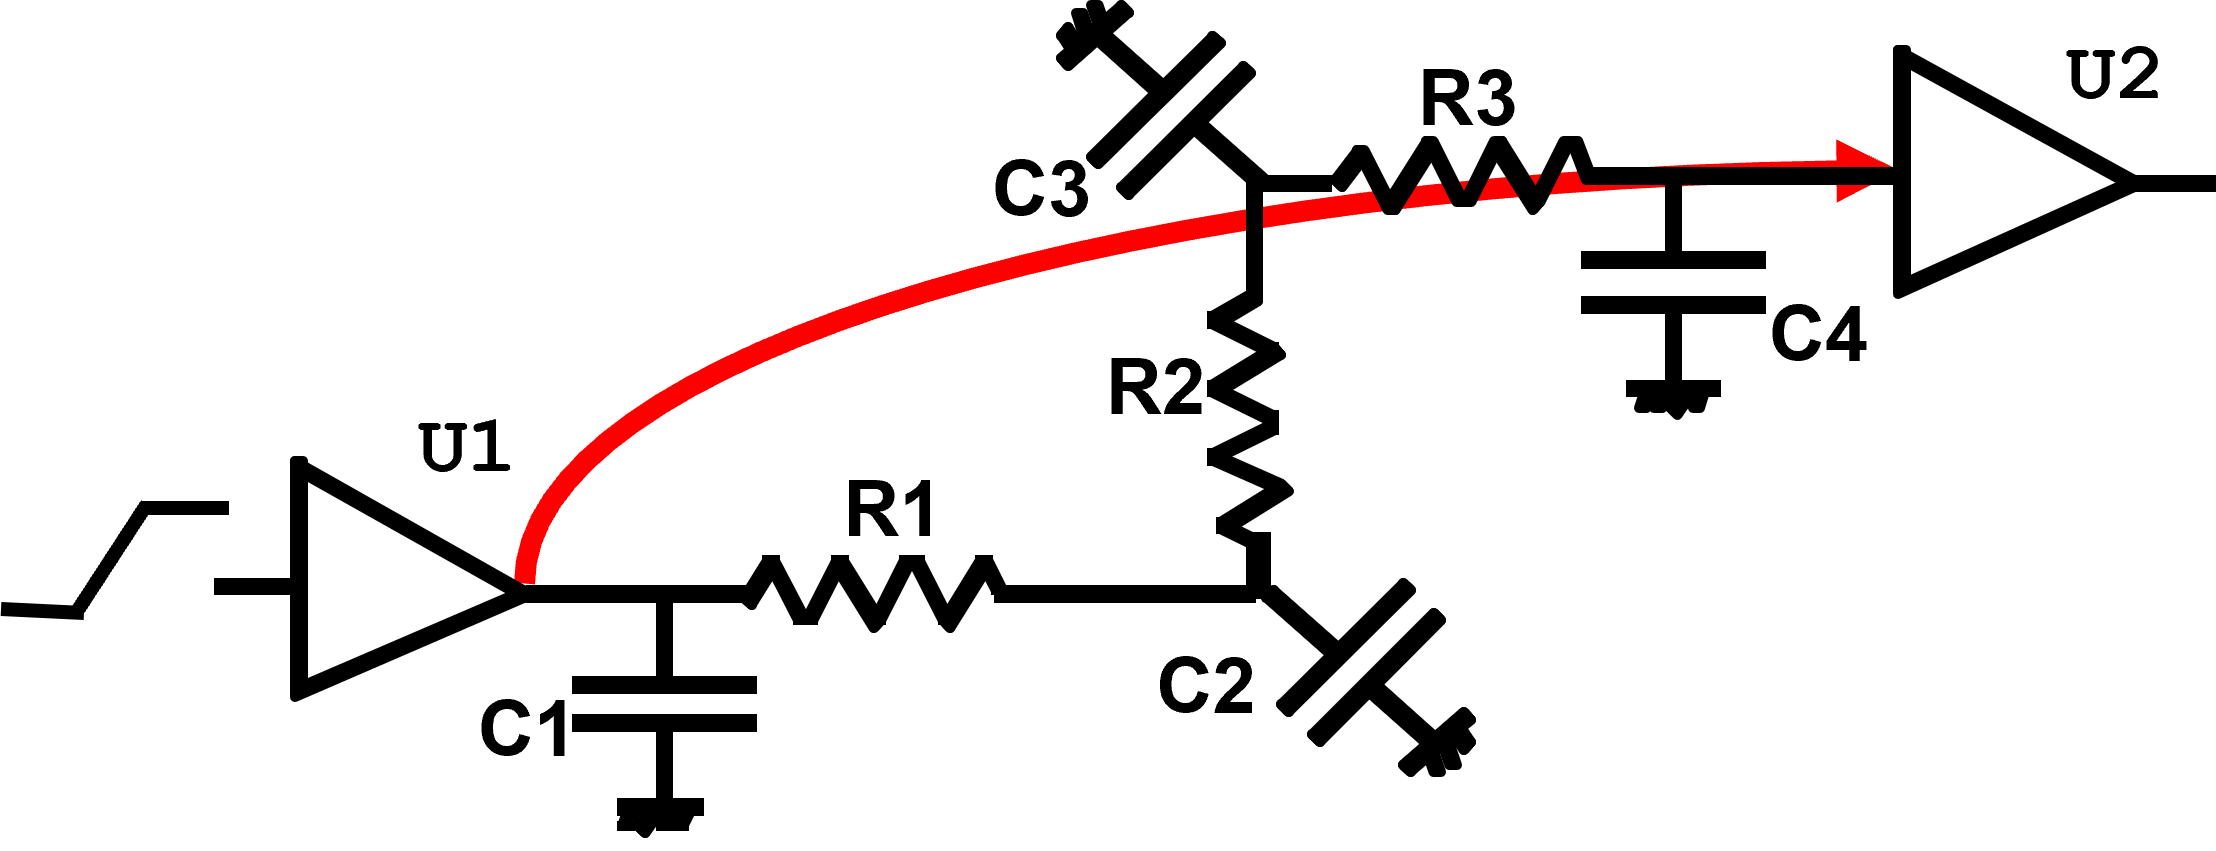
\includegraphics[width=0.4\textwidth]{NET}
		\end{center}
		\begin{itemize}	
		\item \textbf{Calculating \textcolor{red}{Net Delay} is done using Delay Calculation algorithms: Elmore, Arnoldi}
	\end{itemize}
\end{frame}
\begin{frame}
	\frametitle{PreRoute Delay Calculation Algorithm}
	\begin{center}
		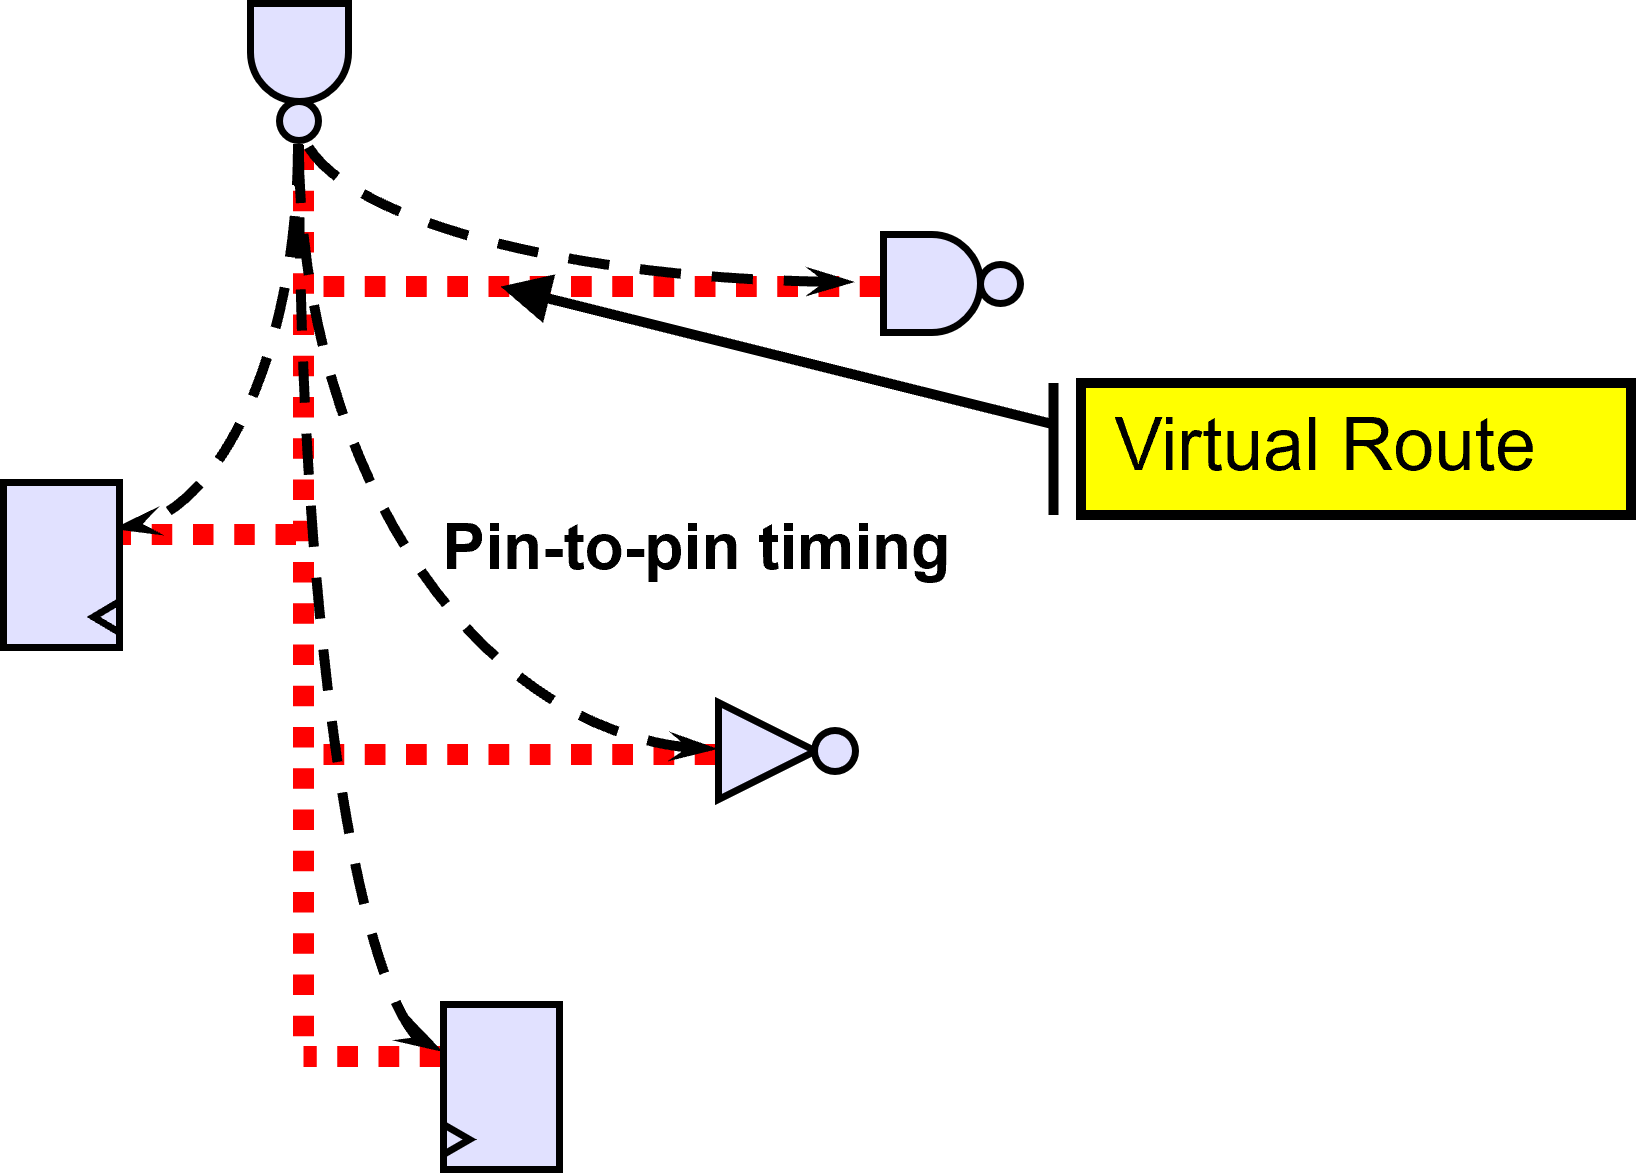
\includegraphics[width=0.6\textwidth]{ELMORE}
	\end{center}
	\begin{itemize}
		\item \textbf{Prior to routing, net geometry is estimated based on a Virtual Route}
		\item \textbf{Since Virtual Routing is only an estimate,an \textcolor{blue}{Elmore} model is used for delay calculation}
		
	\end{itemize}
\end{frame}
\begin{frame}
	\frametitle{PostRoute Delay Calculation Algorithms}
	\begin{center}
		\includegraphics[width=0.4\textwidth]{Arnoldi}
	\end{center}
	\begin{itemize}
		\item \textbf{After routing, detailed nets are available and extraction can be more accurate}
		\item \textbf{By default, Elmore is still used}
		\item \textbf{\textcolor{red}{Arnoldi} can be turned on for postroute calculations}
		
	\end{itemize}	
\end{frame}

	%------------------------------------------------
	\subsection[Intro]{Introduction}
	\begin{frame}
		\frametitle{What is a Standard Cell Library?}
		\begin{columns}	
			\column{0.7\textwidth}
			\begin{itemize}
				\item A Standard Cell is a predesigned
				layout of one specific basic logic gate
				\item Each cell usually has the same
				standard height.
				\item A Standard Cell Library contains a
				varied collection of standard cells
				\item Libraries are usually supplied by an ASIC vendor or library group
			
			\end{itemize}
			\column{0.5\textwidth}
			\begin{center}
				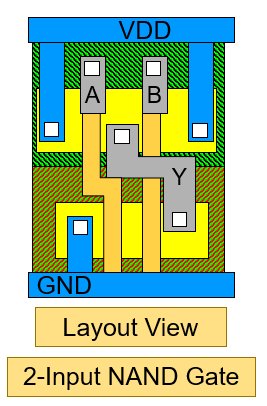
\includegraphics[width=0.8 \textwidth]{Layout View}
			\end{center}
		\end{columns}
	\end{frame}
%--------------------------------------------------
\begin{frame}
	\frametitle{“Layout” vs. “Abstract” Views}
		\begin{itemize}
			\item A standard cell library also contains a corresponding	abstract view for each layout view
			\item Abstract views contain only the minimal data needed
			for Place \& Route
		\end{itemize}
		\begin{center}
			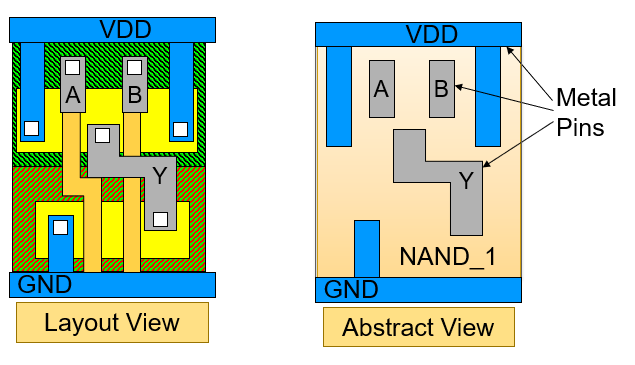
\includegraphics[width=0.85\textwidth]{Frame}
		\end{center}
\end{frame}
%--------------------------------------------------
\begin{frame}
	\frametitle{What Does “Place and Route” Do?}
		\begin{itemize}
			\item Layout is built with three types of reference cells:
				\begin{itemize}
					\item Macro cells (ROMs, RAMs, IP blocks)
					\item Standard cells (nand2, inv, dff, ...)
					\item Pad cells (input, output, bi-dir, Vdd, Vss pads)
				\end{itemize}
			\item You have to define Macro and Pad cell locations during the
			Floorplanning stage, before Placement and Routing
			\item  Location of all Standard Cells is automatically chosen by the tool
			during Placement, based on routability and timing
			\item  Pins are then physically connected during Routing, based on
			timing
		\end{itemize}
		\begin{center}
			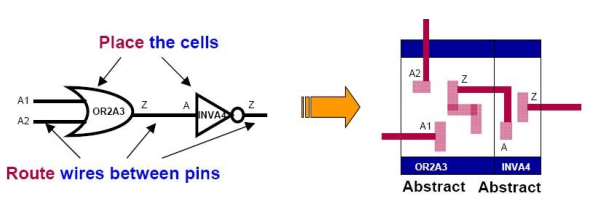
\includegraphics[width=0.65\textwidth]{PnR}
		\end{center}
\end{frame}
%----------------------------------------------------
\begin{frame}
	\frametitle{Timing-Driven Placement}
	\begin{itemize}
		\item Standard cells are placed in “placement rows”
		\item Cells in a timing-critical path are placed close together to reduce routing-related delays, which is \textcolor{red}{Timing-Driven Placement}
	\end{itemize}
	\begin{center}
		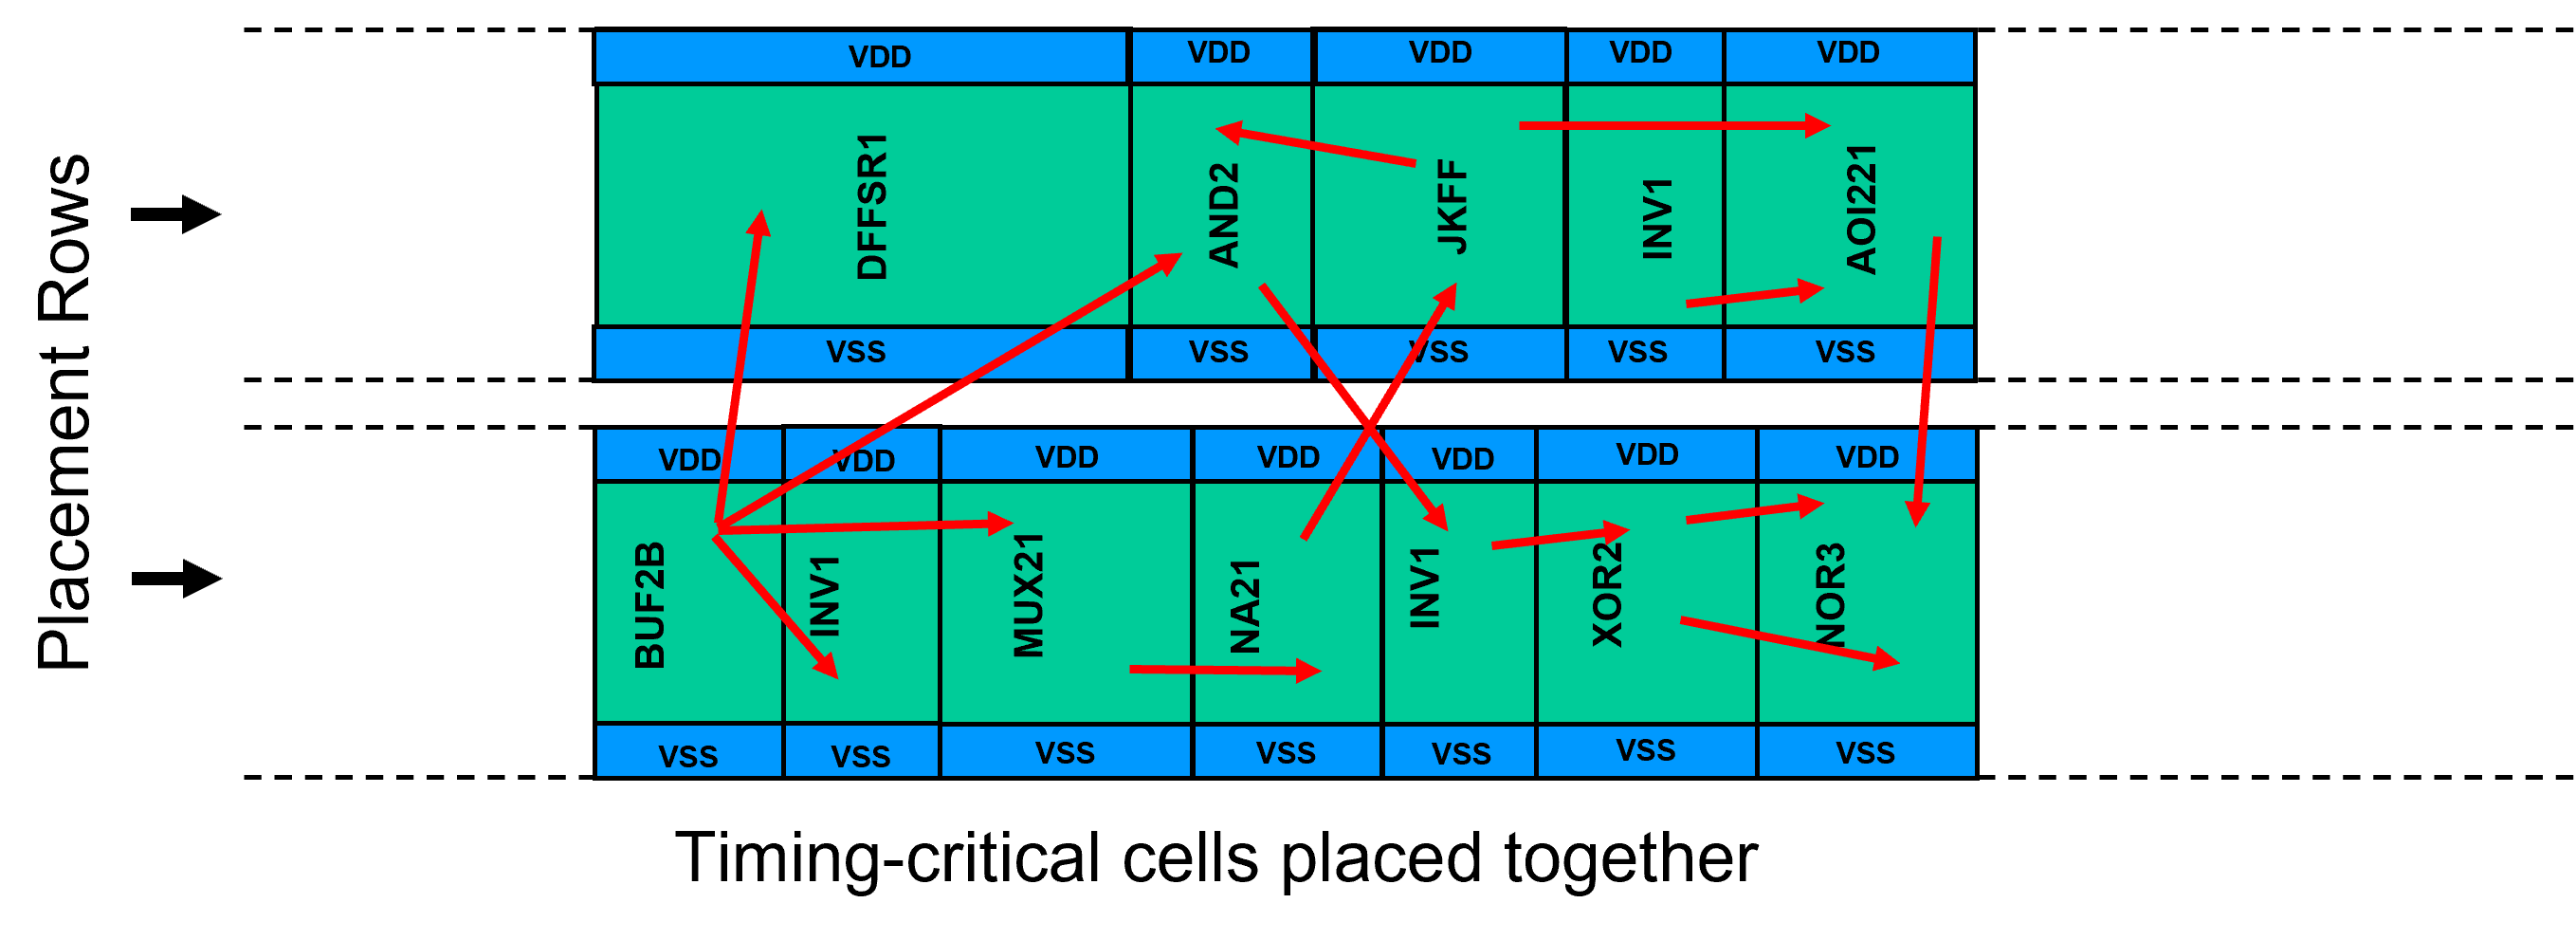
\includegraphics[width=0.9\textwidth]{TDP}
	\end{center}
\end{frame}
%--------------------------------------------------
	\begin{frame}
		\frametitle{Abutted Rows}
		\begin{itemize}
			\item Placement rows are
			commonly abutted to reduce core area
			\item Cell orientations in abutted
			rows are flipped
		\end{itemize}
		\begin{center}
			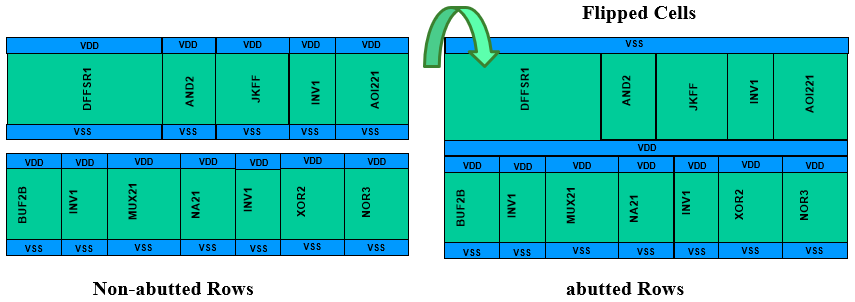
\includegraphics[width=0.8\textwidth]{CELL}
		\end{center}
	\end{frame}
%--------------------------------------------------
	\begin{frame}
		\frametitle{Vias: Connecting Metal to Metal}
			\begin{itemize}
				\item Connecting between metal layers requires one or more vias.
				\begin{example}
					Connecting a signal from Metal 1 to Metal 3 requires
					two vias and an intermediate Metal 2 connection
				\end{example}
			\end{itemize}	
			\begin{center}
				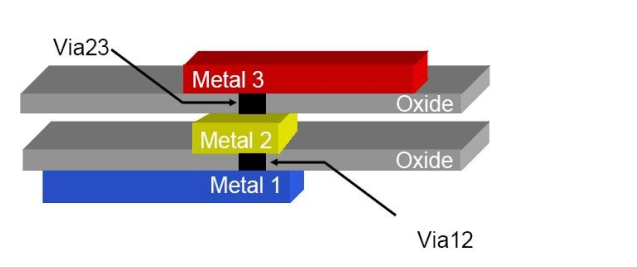
\includegraphics[width=0.9\textwidth]{VIA}
			\end{center}
	\end{frame}
%--------------------------------------------------
\begin{frame}
	\frametitle{Preferred Routing Directions}
	\begin{columns}	
		\column{0.7\textwidth}
		\begin{itemize}
			\item Metal layers have preferred
			routing directions
			\item Default preferred direction:
				\begin{itemize}
					\item \textcolor{blue}{Metal 1 – Horizontal}
					\item \textcolor{yellow}{Metal 2 – Vertical}
					\item \textcolor{red}{Metal 3 – Horizontal}, etc
				\end{itemize}
			\item \textcolor{red}{Why is this beneficial?}
		\end{itemize}
		\column{0.5\textwidth}
		\begin{center}
			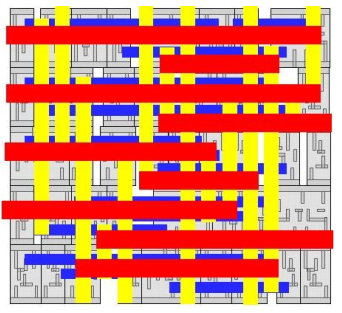
\includegraphics[width=0.7 \textwidth]{routing}
		\end{center}
	\end{columns}
	\pause
	\begin{block}{preferred routing directions}
		Having preferred routing directions greatly reduces the amount of metal layer “jumping” the router
		may need to do to connect any two pins, which reduces resistance and therefore propagation delay,
		as well as run time.
	\end{block}
\end{frame}
%--------------------------------------------------
\begin{frame}
	\frametitle{Routing Tracks}
	\begin{itemize}
		\item Metal routes must meet minimum width and spacing “design rules”
		to prevent open and short circuits during fabrication
		\item In gridded routers these design rules determine the minimum
		center-to-center distance for each metal layer, a.k.a. grid or track
		spacing
		\item Congestion occurs if there are more wires to be routed than
		available tracks
	\end{itemize}
	\begin{center}
		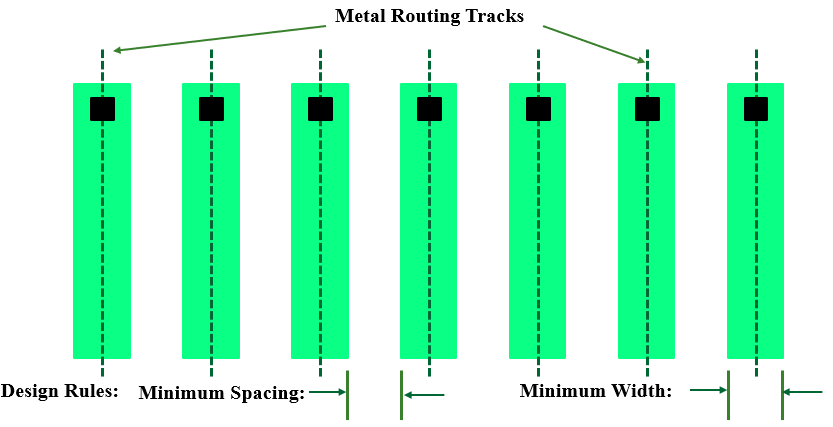
\includegraphics[width=0.7\textwidth]{Tracks}
	\end{center}
\end{frame}
\begin{frame}
	\frametitle{Timing-Driven Routing}
		\begin{itemize}
			\item Routing along the timing-critical path is given priority:
			\begin{itemize}
				\item Creates shorter, faster connections
			\end{itemize}
			\item Non-critical paths are routed around critical areas:
			\begin{itemize}
				\item Reduces routability problems for critical paths
				\item Does not adversely impact timing of non-critical paths
			\end{itemize}
		\end{itemize}
		
		\begin{center}
			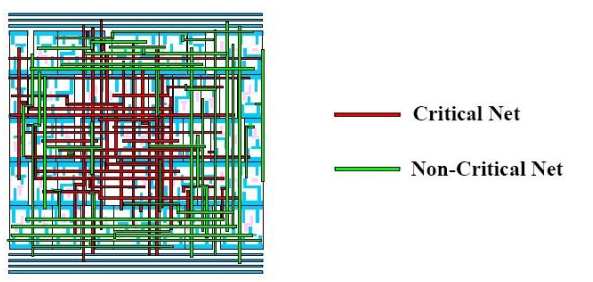
\includegraphics[width=0.7 \textwidth]{Rout-ability }
		\end{center}
\end{frame}
	\begin{frame}
		\frametitle{Logic Optimization}
		What if critical paths do not meet timing/drive requirements,
		even with timing-driven placement or routing?
		\begin{center}
			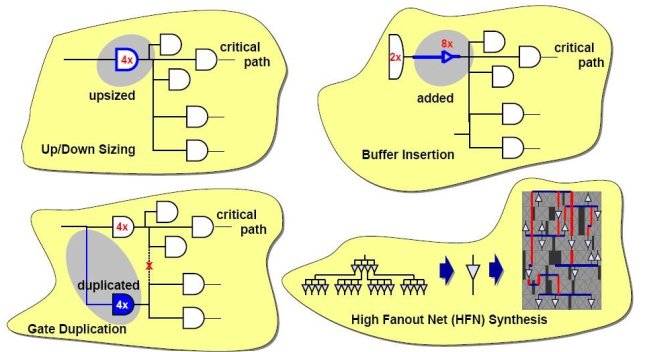
\includegraphics[width=0.8\textwidth]{Logic}
		\end{center}
	\end{frame}
%---------------------------------------------------
\subsection[Appendix A]{Appendix A}
\begin{frame}
	\frametitle{What is a Gate in “Gate-level Netlist”?}
	\textbf{Gate:} Basic Logic Component
	\begin{center}
		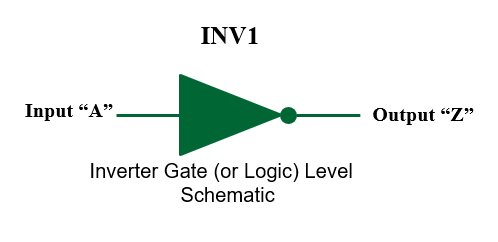
\includegraphics[width=0.8\textwidth]{INV}
	\end{center}
	\begin{itemize}
		\item Other Gates:
				\newline
					Buffer, Nand, Nor, Xor, AOI, Mux, D-FF, Latch, etc
	\end{itemize}
\end{frame}

\begin{frame}
	\frametitle{Transistor or Device Representation}
		\begin{center}
			\textbf{\underline{CMOS Inverter Example}}
			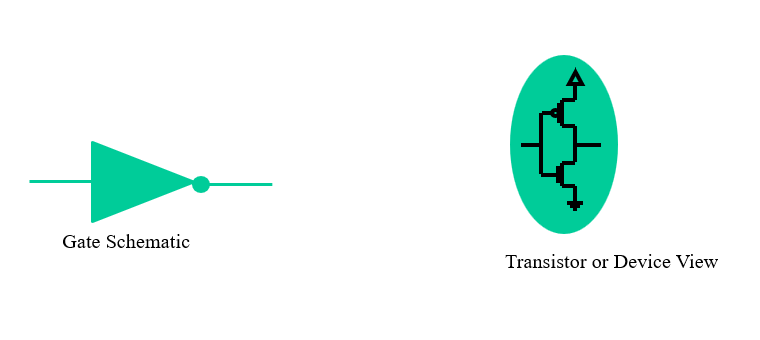
\includegraphics[width=0.8\textwidth]{Inverter}
		\end{center}
			
		\begin{alertblock}	
			
			Gates are made up of active devices or transistors.
		\end{alertblock}
\end{frame}

\begin{frame}
	\frametitle{Basic Devices and Interconnect}
	\begin{itemize}
		\item Integrated circuits are built out of active and passive
		components, also called \underline{devices}:
		\begin{columns}	
			\column{0.3\textwidth}
			\begin{itemize}
				\item Active devices:
				\begin{itemize}
					\item Transistors
					\item Diodes
				\end{itemize}
				\item Passive devices:
				\begin{itemize}
					\item Resistors
					\item Capacitors
				\end{itemize}
			\end{itemize}
			\column{0.5\textwidth}
			\begin{center}
				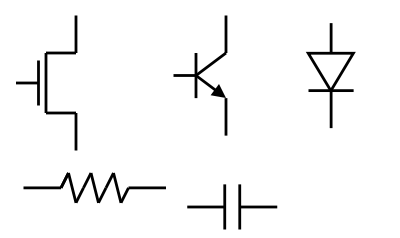
\includegraphics[width=0.5 \textwidth]{Devices }
			\end{center}
		\end{columns}
		\item Devices are connected together with polysilicon or
		metal interconnect:
		\begin{itemize}
			\item Interconnect can add unwanted or \underline{parasitic} capacitance,
			resistance and inductance effects
		\end{itemize}
	\item Device types and sizes are \underline{process} or \underline{technology}
	specific:
		\begin{itemize}
			\item The focus here is on CMOS technology
		\end{itemize}
	\end{itemize}
\end{frame}

\begin{frame}
	\frametitle{What is “Physical Layout”?}
		\begin{center}
			\textbf{\underline{CMOS Inverter Example}}
			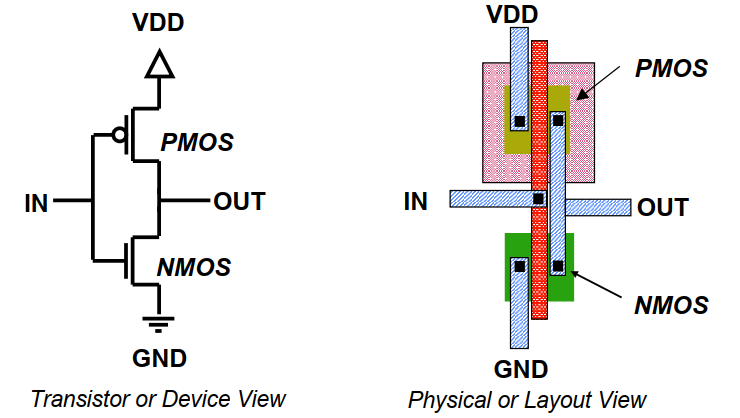
\includegraphics[width=0.8\textwidth]{CMOS}
	\end{center}
\textbf{Physical Layout – Topography of \underline{devices} and \underline{interconnects}, made
	up of \underline{polygons} that represent different \underline{layers of material}.	}
\end{frame}

\begin{frame}
	\frametitle{Process of Device Fabrication}
	\begin{itemize}
		\item Devices are fabricated vertically on a silicon substrate wafer by
		layering different materials in specific locations and shapes on
		top of each other
		\item Each of many process \textbf{\underline{masks}} defines the shapes and locations
		of a specific layer of material (diffusion, polysilicon, metal,
		contact, etc)
		\item Mask shapes, derived from the layout view, are transformed to
		silicon via photolithographic and chemical processes
	\end{itemize}
\begin{center}
	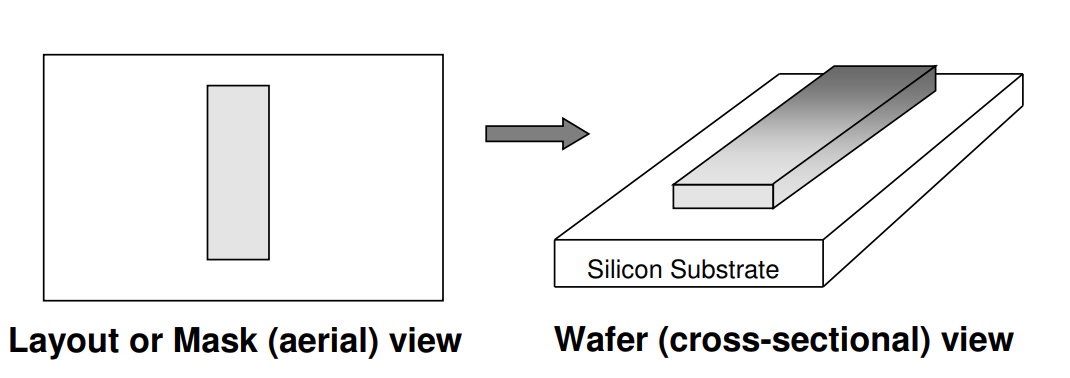
\includegraphics[width=0.7\textwidth]{wafer}
\end{center}
\end{frame}

\begin{frame}
	\frametitle{Wafer Representation of Layout Polygons}
	\textbf{Example of complimentary devices in 0.25 um CMOS
	\underline{technology} or \underline{process}.}
	\begin{center}
		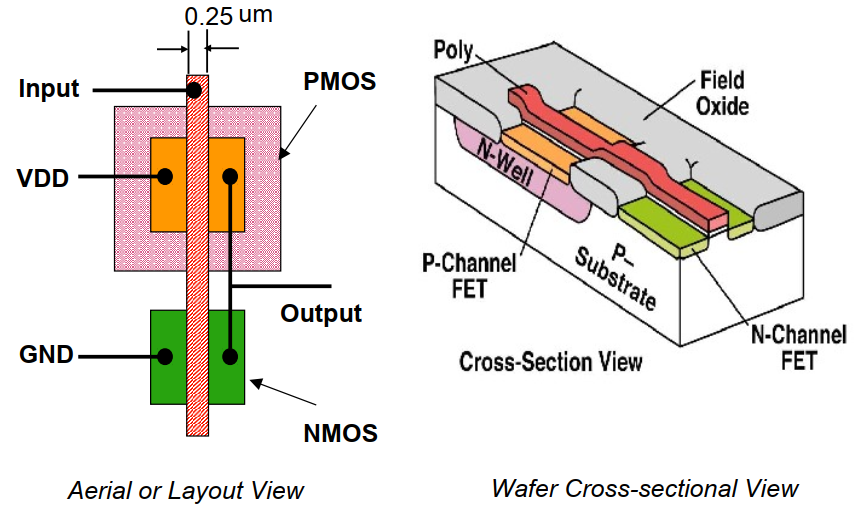
\includegraphics[width=0.9\textwidth]{Polygons}
	\end{center}
\end{frame}

\begin{frame}
	\frametitle{What is Meant by “0.xx um Technology”?}
	\textbf{Gate or Channel\underline{} Dimensions (L and W)}
		\begin{center}
		\includegraphics[width=0.5\textwidth]{Channel}
		\end{center}
	\begin{block}{0.xx um Technology}
		\begin{itemize}
			\item In CMOS Technology the um or nm dimension refers to the channel length,
			a minimum dimension which is fixed for most devices in the same library.
			\item Current flow or drive strength of the device is proportional to W/L;
			Device size or area is proportional to W x L.
		\end{itemize}
	\end{block}
\end{frame}

\begin{frame}
	\frametitle{Comparing Technologies}
		\begin{center}
			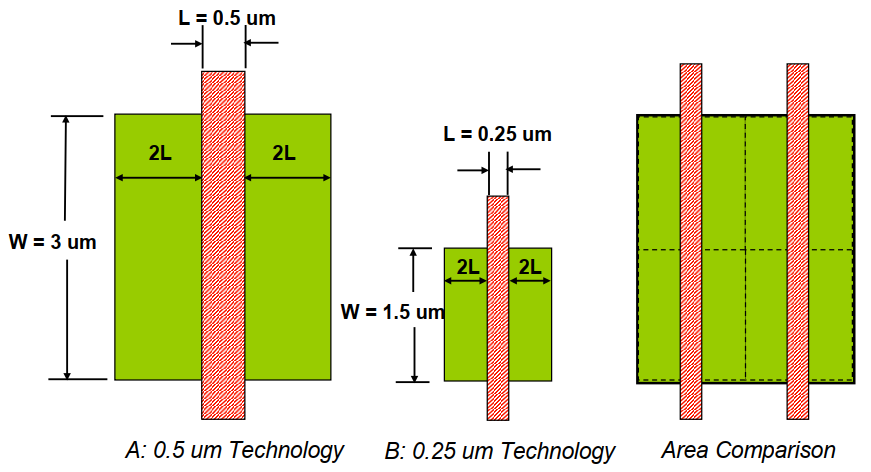
\includegraphics[width=0.7\textwidth]{Drive_strength}
		\end{center}
		\textbf{The drive strength of both devices is the same: W/L = 6}.
		\newline
	\textbf{	The diffusion area (5xLxW) of A is 4x that of B}.\newline
		\textbf{Which is preferred?}
\end{frame}

\begin{frame}
	\frametitle{Relative Device Drive Strengths}
		\begin{center}
			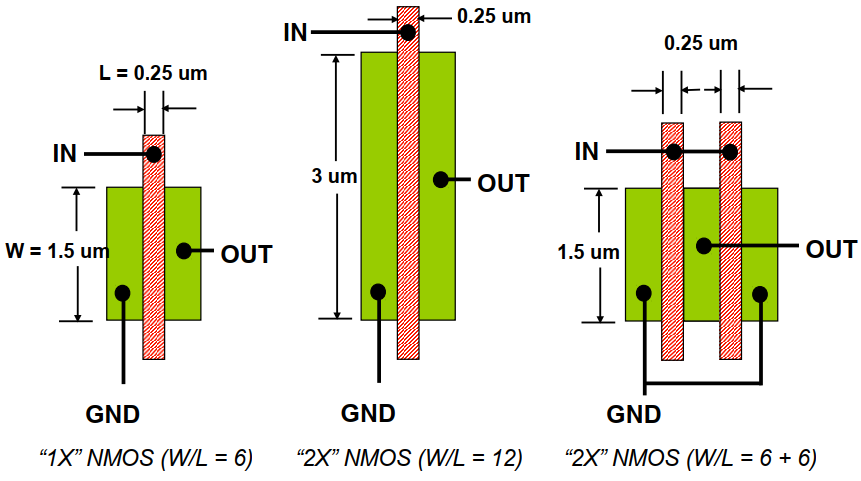
\includegraphics[width=0.7\textwidth]{Strengths}
		\end{center}
	\begin{block}{ Drive Strengths}
		To double the drive strength of a device, double the channel width
	(W), or connect two 1X devices in parallel. The latter approach keeps
	the height at a fixed or “standard” height.
	\end{block}
\end{frame}

\begin{frame}
	\frametitle{Gate Drive Strength Example}
	
	\begin{center}
		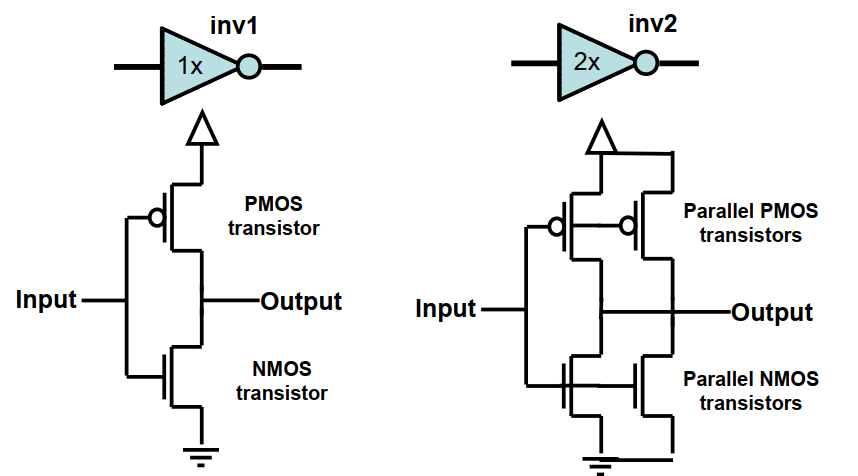
\includegraphics[width=0.7\textwidth]{Gate Drive}
	\end{center}
\begin{block}{Gate Drive}
	Each gate in the library is represented by multiple cells with
	different drive strengths for effective speed vs. area optimization.
\end{block}
\end{frame}

\begin{frame}
	\frametitle{Drive/Buffering Rules: Max Transition/Cap}
	\begin{center}
		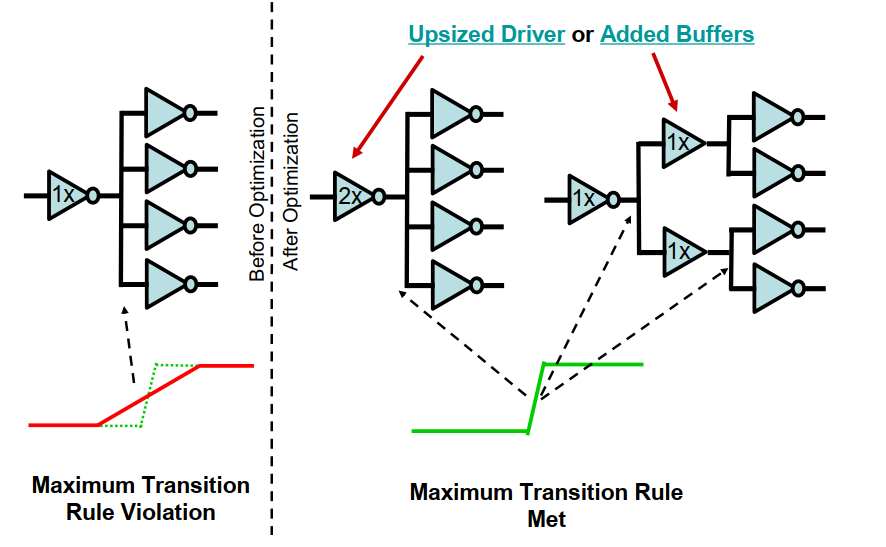
\includegraphics[width=\textwidth]{Rules}
	\end{center}
\end{frame}
%---------------------------------------------------
\section[Floor]{Floorplanning}
\subsection[Floor]{Floorplanning}
\begin{frame}
	\frametitle{What Is Floorplanning?}
	\begin{block}{Definition}
		Floorplanning is the process of deriving the die size, allocating space for soft blocks, planning power, and macro placement.
	\end{block}
	\begin{columns}	
		\column{0.5\textwidth}
		With a top-level netlist, you can start to floorplan the chip.
		\begin{itemize}
			\item Define Die Size.
			\item Place the IOs.
			\item Perform macro placement.
			\item Perform power planning.
			\item Power domain definition
			\item Flip-chip bump placement
		\end{itemize}
		\column{0.6\textwidth}
		\begin{center}
			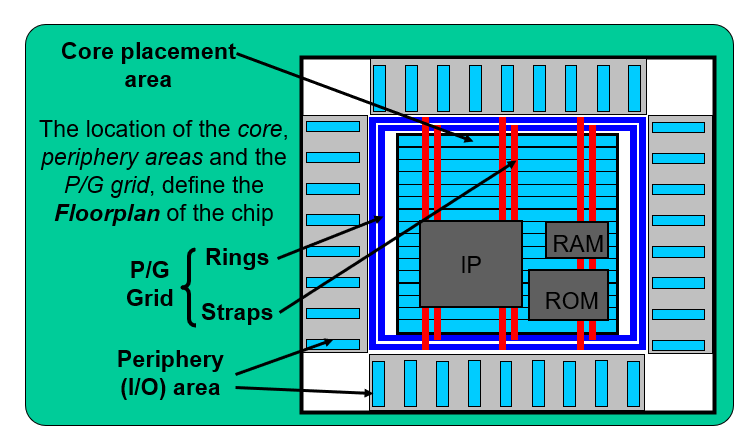
\includegraphics[width= \textwidth]{Floorplanning1}
		\end{center}
	\end{columns}
\end{frame}
	\begin{frame}
		\frametitle{Floorplanning}
		\begin{itemize}
			\item Floorplanning consists of defining the \textcolor{red}{Core Placement area}, the \textcolor{red}{Periphery area} and the \textcolor{red}{Power/Ground grid}.
			\item The Core Placement area consists of \textcolor{red}{Placement Rows} where standard cells and macro cells are
			placed.
			\item A placement row consists of a row of \textcolor{red}{“unit tile”} cells (part of the standard cell library, width
			defined by the minimum metal pitch). Standard cells are placed in the core of a chip and occupy
			specific tile(s) within the placement rows. \textcolor{red}{A standard cell may occupy a single or multiple tiles}.
			\item The pad cells (\textcolor{red}{input, output, bi-dir, power and ground pads}) are placed in the Periphery Area,
			which is defined by the area around the outside boundary of the core, usually separated by a
			“core-to-pad” spacing distance.
		\end{itemize}
	\end{frame}
\begin{frame}
	\frametitle{What Are Sites and Rows?}
	\begin{block}
	
	A site is the minimum unit of placement. It represents a slot where a cell can be placed.
	Rows are multiples of sites and define locations where the placement tool places cells.
	\end{block}
Placement tools place cells in locations defined by the cell’s description in the LEF file. If a cell is of type
CORE, then it can only be placed in a CORE rows. If a cell is of type IO, it can only be placed in IO rows
\begin{center}
	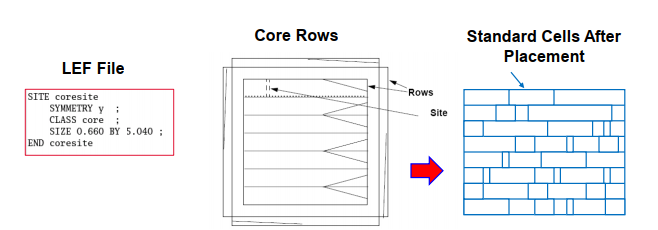
\includegraphics[width=0.8\textwidth]{SITE}
\end{center}
\end{frame}
%---------------------------------------------------
\begin{frame}
	\frametitle{Core and IO Region}
	\begin{itemize}
		\item \textbf{From:}
			\begin{itemize}
				\item  A gate level netlist
				\item Relevant physical libraries
				\item Default or user specified aspect ratio and utilization.
			\end{itemize}
		\item \textbf{Calculate the area of all macro cells and leaf cells}
		\item \textbf{Generate bounding shapes and cell placement rows}
		\item \textbf{Place IO PADs}
			\begin{itemize}
				\item Signal pads
				\item Filler and corner pads
				\item Bump or flip-chip IO pads
			\end{itemize}
	\end{itemize}
	 \begin{equation}    % <--- deleted empty lines
		\textbf{Utilization} = \frac{(\textbf{Total Std Cell} \textbf{\textbf{+}} \textbf{Macro Cell Area})}{\textbf{Core Area}} \textbf{* 100\%}
	\end{equation}
\end{frame}
%------------------------------------------
\begin{frame}
	\frametitle{Utilization: A Factor in Determining Core Size}
	\begin{columns}	
		\column{0.5\textwidth}
		\begin{itemize}
			\item Core “utilization” is the
			percentage of the core that is
			used by placed std cells and
			macros
			\item Ideally would like to achieve
			100\% utilization at tape-out. In
			practice range is 80-85%
			\item Recommended starting netlist
			utilization should not exceed
			60-75% to allow for logic
			optimizations and DFM
		\end{itemize}
		\column{0.5\textwidth}
		\begin{center}
			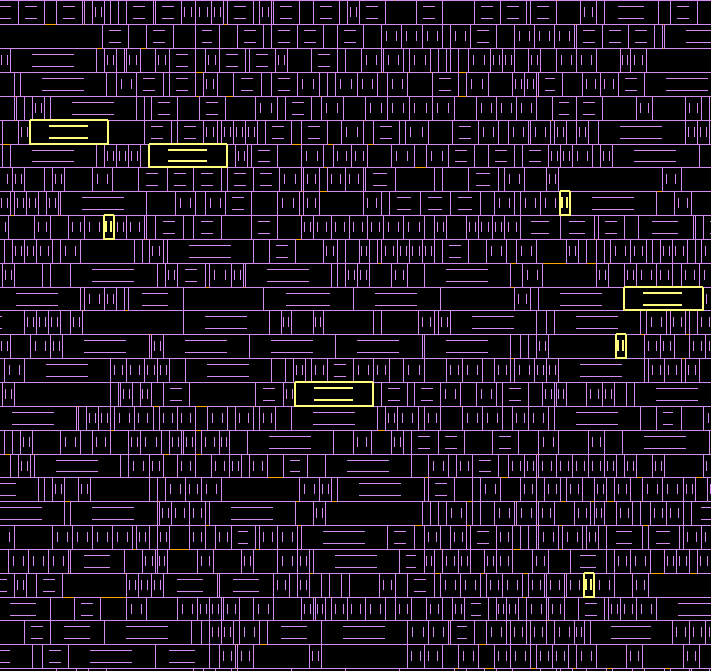
\includegraphics[width=0.8 \textwidth]{Utilization}
		\end{center}
	\end{columns}
		 \begin{equation}    % <--- deleted empty lines
		\textbf{Utilization} = \frac{(\textbf{Total Std Cell} \textbf{\textbf{+}} \textbf{Macro Cell Area})}{\textbf{Core Area}} \textbf{* 100\%}
	\end{equation}
\end{frame}
\begin{frame}
	\frametitle{Aspect Ratio: A Factor in Determining Core Size}
		\begin{itemize}
			\item \textbf{Aspect ratio} is the ratio between vertical routing resources to horizontal routing resources.
			\item If you specify a ratio of 1.00, the height and width are the same and therefore the core is a square.
			\item If you specify a ratio of 2.00, the height is two times the width.
		\end{itemize}
	\begin{center}
		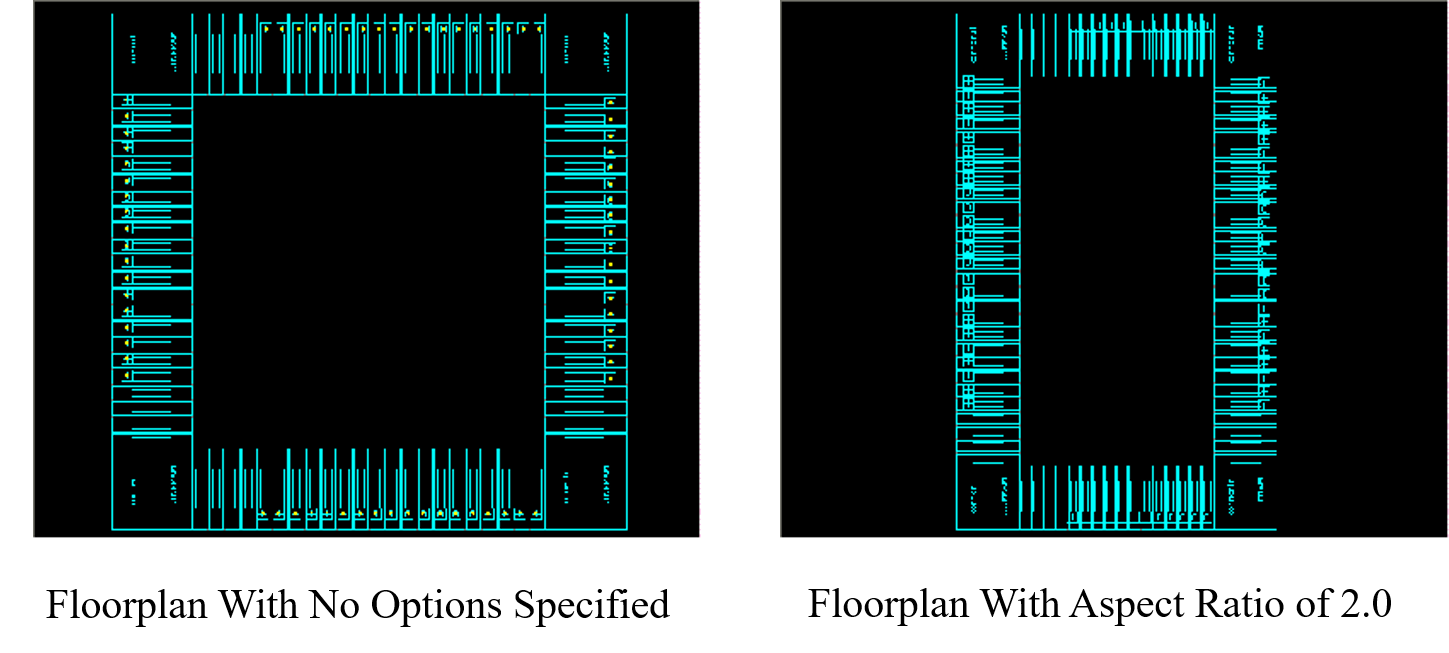
\includegraphics[width=0.7\textwidth]{aspectratio}
	\end{center}
\end{frame}	
\begin{frame}
	\frametitle{Balance Routing Resources}
		\begin{itemize}
			\item  If less vertical routing resources are available,
			make floorplan \underline{wider} (aspect ratio $<$ 1) if possible,
			to increase vertical routing resources
			\item If less horizontal routing resources are available,
			make floorplan \underline{taller} (aspect ratio $>$ 1) if possible,
			to increase horizontal routing resources
		\end{itemize}
	\begin{block}{Note}
		Balancing vertical/horizontal routing resources
		reduces overall congestion
	\end{block}
\end{frame}	
\begin{frame}
	\frametitle{Pad-Limited Design}
		\begin{center}
		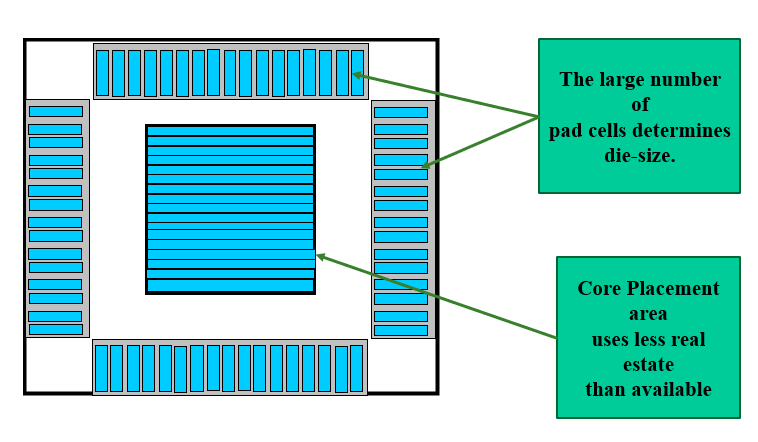
\includegraphics[width=0.7\textwidth]{Pad-Limited}
	\end{center}
	\begin{alertblock}{Question}
		If the utilization of a pad-limited design is too high
		during floorplanning will reducing it affect die size?
	\end{alertblock}
\end{frame}

\begin{frame}
	\frametitle{Core-Limited Design}
		\begin{center}
			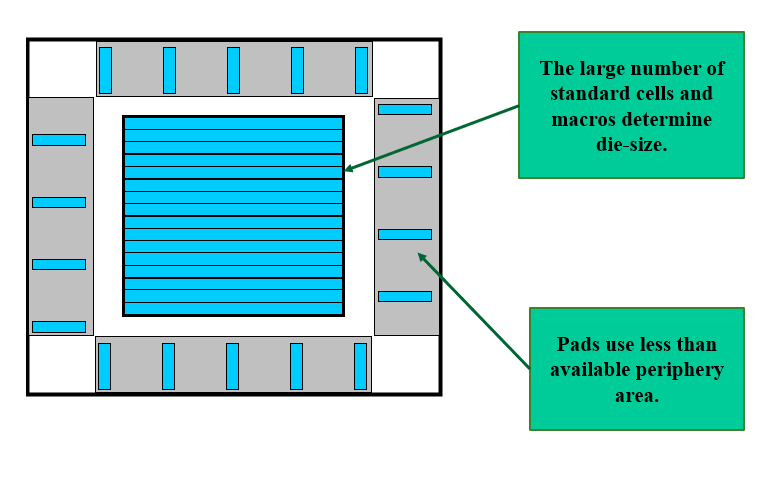
\includegraphics[width=0.7\textwidth]{Core-Limited}
		\end{center}
	\begin{alertblock}{Question}
		If the utilization of a core-limited design is too high
		during floorplanning will reducing it affect die size?
	\end{alertblock}
\end{frame}
%---------------------------------------------
\subsection[Macro]{Hard Macro Placement}
	\begin{frame}
		\frametitle{Hard Macro Placement}
		\begin{itemize}
			\item When placing large macros we must consider impacts on routing,
			timing and power. Usually \textcolor{blue}{push them to the sides} of the floorplan.
				\begin{itemize}
					\item Placement algorithms generally perform better with a
					\textcolor{green}{single large rectangular placement area}
					\item For wire-bond place power hungry macros \textcolor{blue}{away from the chip center}
				\end{itemize}
			\item After placing hard macros, mark them as \textcolor{blue}{FIXED}.
		\end{itemize}
		\begin{center}
			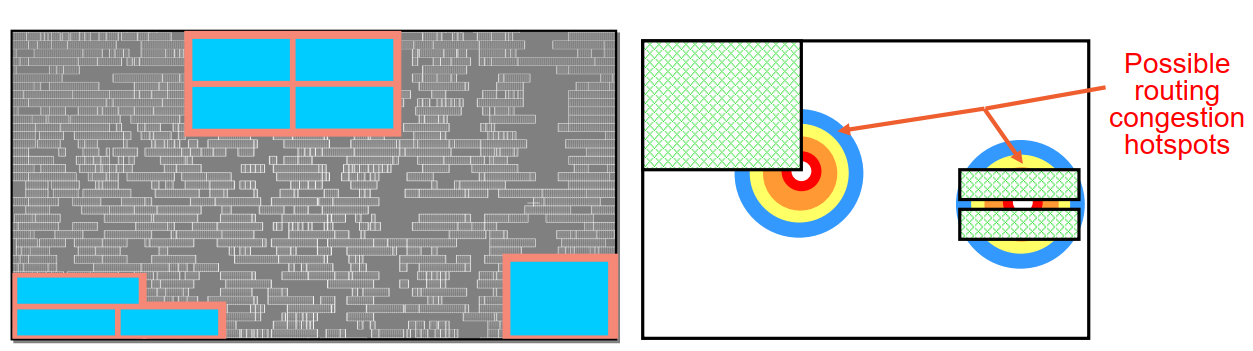
\includegraphics[width=0.9\textwidth]{Hard Macro}
		\end{center}
	\end{frame}
\begin{frame}
	\frametitle{Placement Bounds}
	\frametitle{Placement Blockages and Halos}
	\begin{columns}	
		\column{0.7\textwidth}
		\begin{itemize}
			\item Sometimes, we want to “help” the tool put certain
			logic in certain regions or cluster them together.
			\item Place and Route tools define several types of placement bounds:
			\begin{itemize}
				\item \textcolor{red}{\textbf{Soft move bounds}} specify placement goals, with no guarantee that the cells will be placed inside the    bounds.
				\item \textcolor{red}{\textbf{Hard move bounds}} force placement of the specified cells inside the bounds.
				\item \textcolor{red}{\textbf{Exclusive move bounds}} force the placement of the specified cells inside the bounds. All other cells must be placed outside the bounds.
			\end{itemize}
		\end{itemize}
		\column{0.5\textwidth}
		\begin{center}
			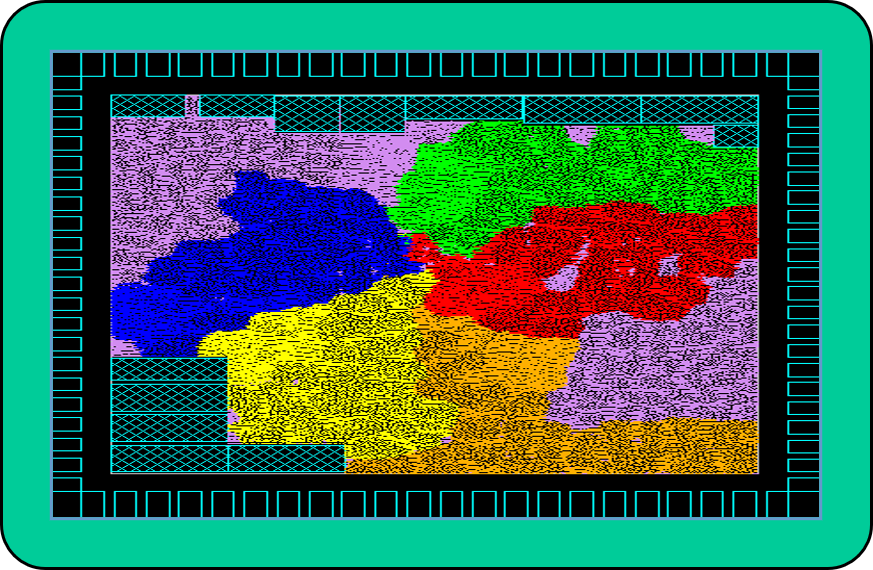
\includegraphics[width= 0.8\textwidth]{before}\qquad
			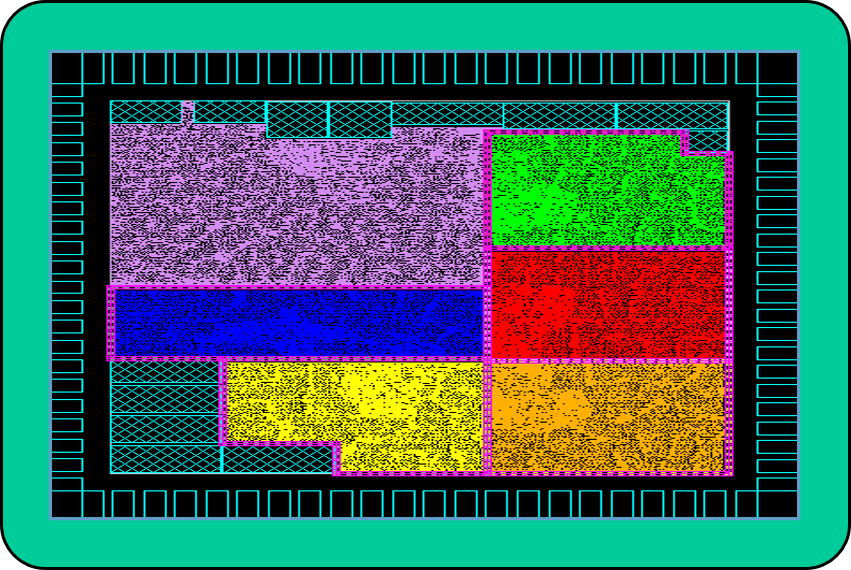
\includegraphics[width=0.8\textwidth]{after}
		\end{center}
	\end{columns}
\end{frame}
\begin{frame}
	\frametitle{Placement Blockages and Halos}
			\begin{columns}	
		\column{0.6\textwidth}
		\begin{itemize}
			\item Placement blockage \textcolor{blue}{halos} are areas that the tools should not place any cells.
			\item  These, too, have several types:
				\begin{itemize}
					\item \textcolor{red}{\textbf{Hard Blockage}} – no cells can be placed
					inside.
					\item \textcolor{red}{\textbf{Soft Blockage}} – cannot be used during
					placement, but may be used during
					optimization.
					\item \textcolor{red}{\textbf{Partial Blockage}} – an area with lower
					utilization.
					\item \textcolor{red}{\textbf{Halo (padding)}} – an area outside a
					macro that should be kept clear of
					standard cells
				\end{itemize}
		\end{itemize}
		\column{0.5\textwidth}
		\begin{center}
			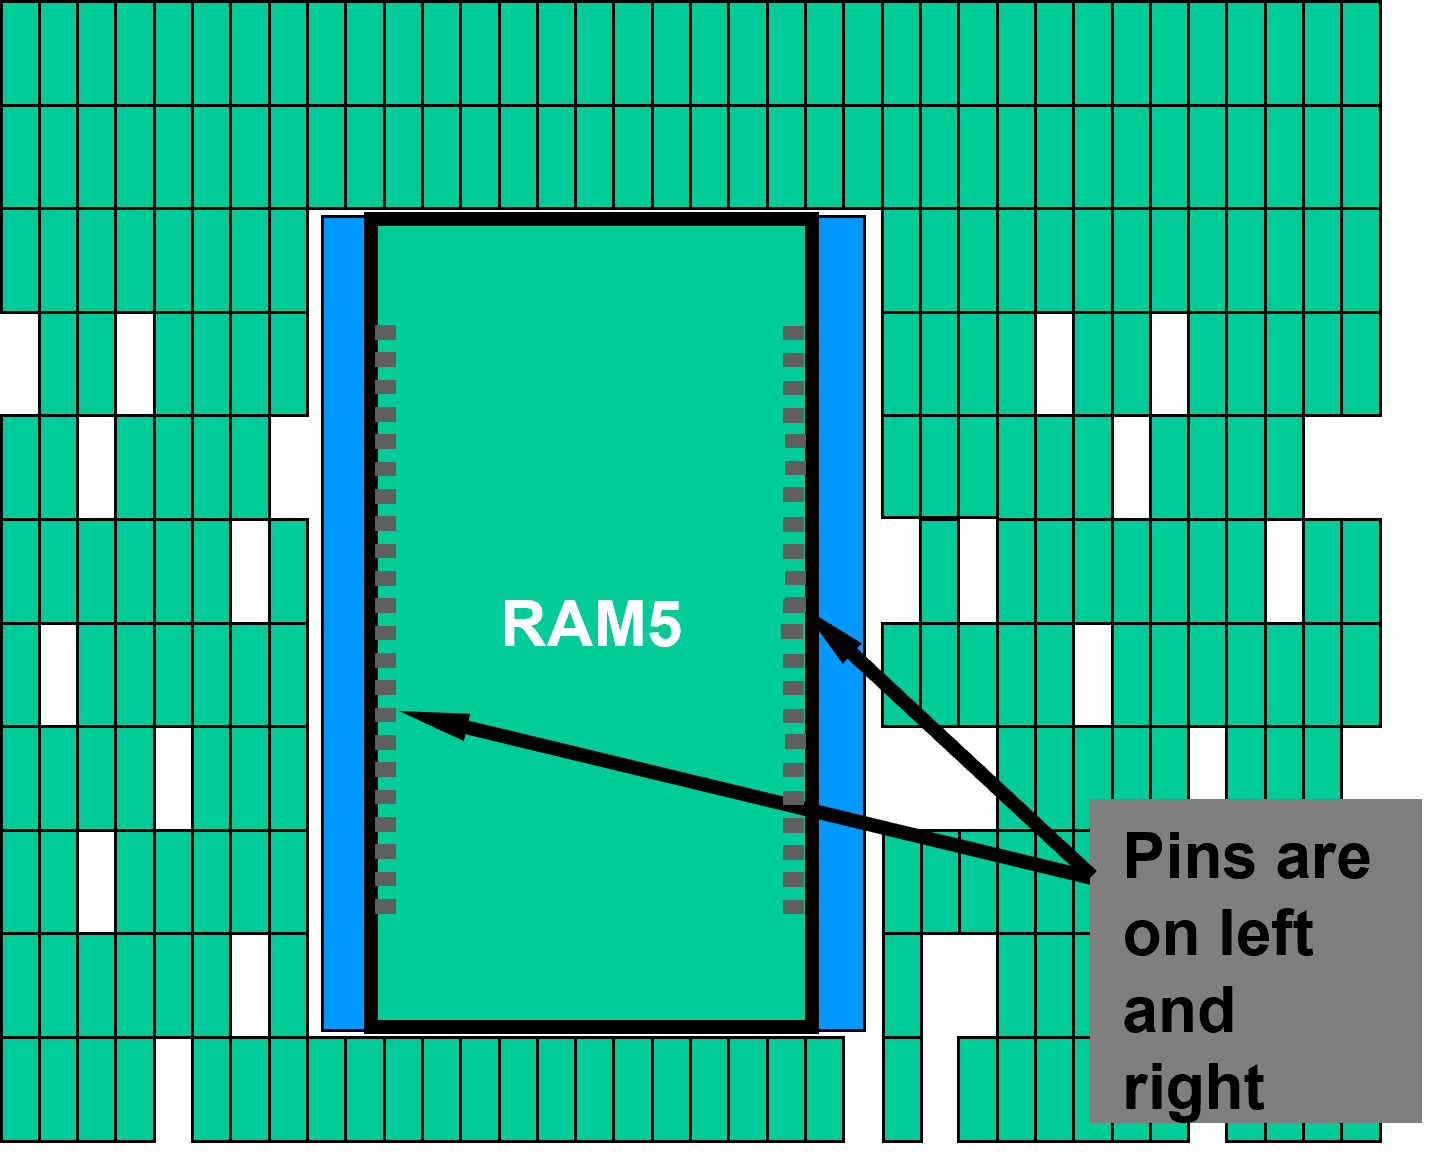
\includegraphics[width= \textwidth]{Padding}
		\end{center}
	\end{columns}
\end{frame}
\begin{frame}
	\frametitle{Placement Blockages: Macro Keepout Margin (Padding)}
	\begin{block}{Padding}
		A keepout margin is a region around the boundary of fixed macros in the design in which no other cells are placed.
	\end{block}
	\begin{center}
		\includegraphics[width=\textwidth]{keepout}
	\end{center}
\end{frame}
\begin{frame}
	\frametitle{Placement Blockages: Adding or Modifying Global Placement Blockages}
	\begin{center}
		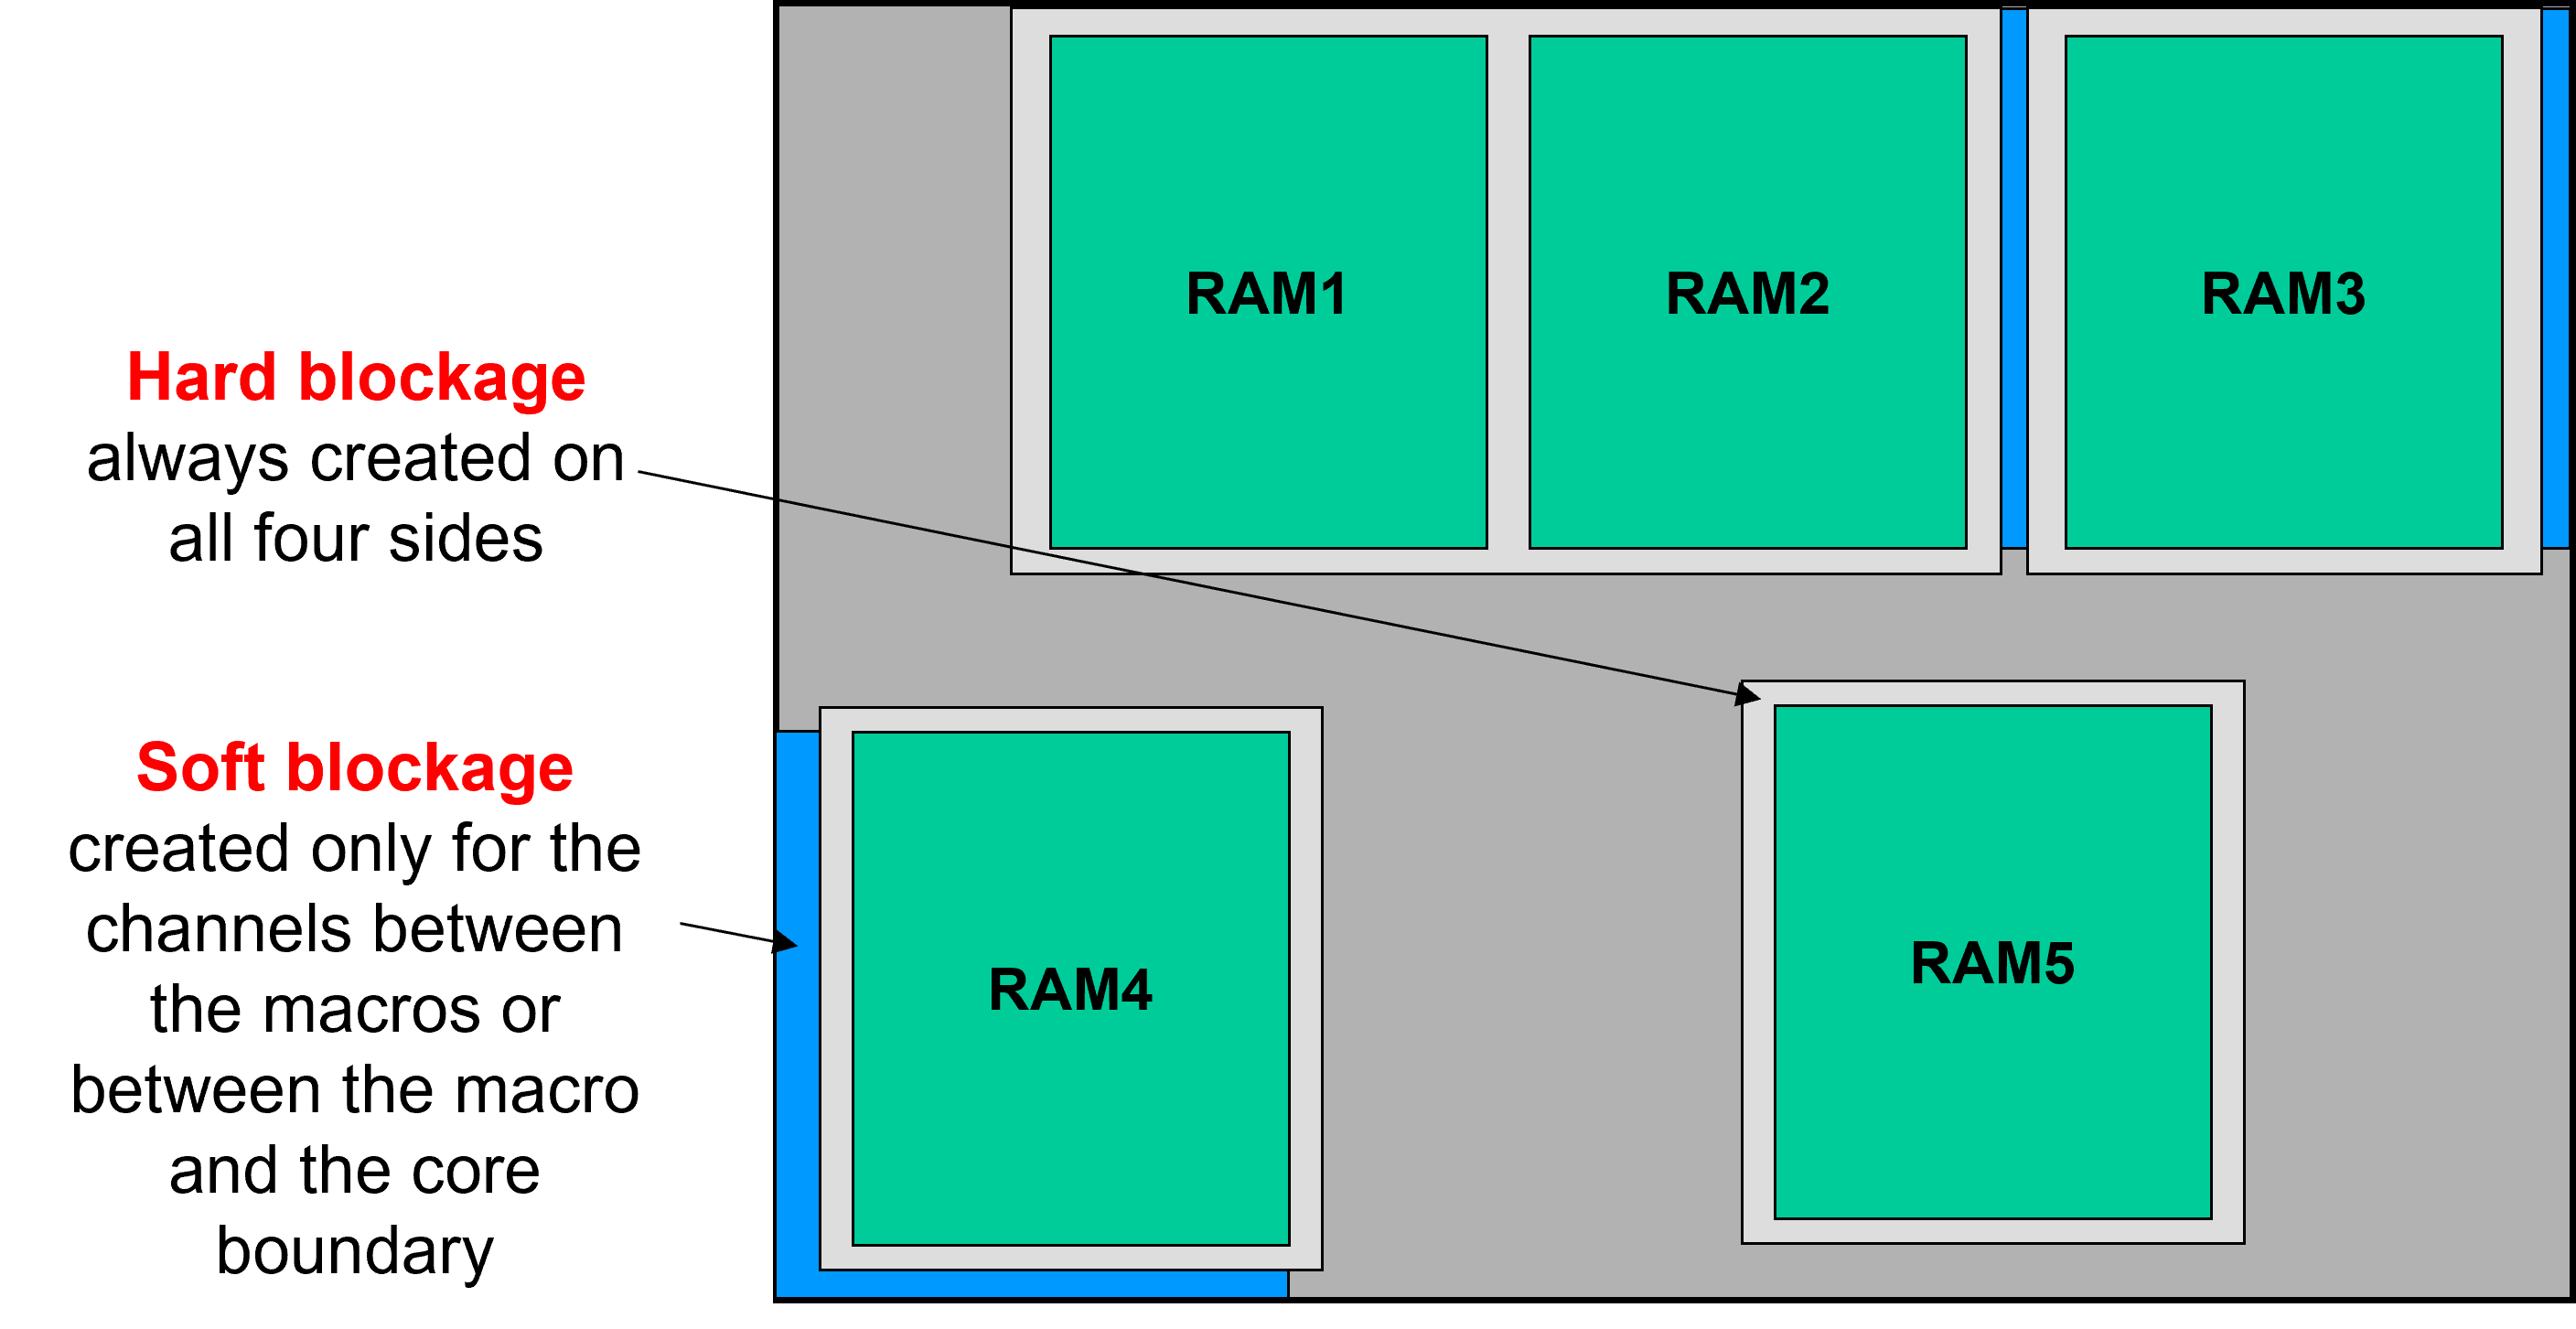
\includegraphics[width=\textwidth]{Blockage}
	\end{center}
\end{frame}
\begin{frame}
	\frametitle{Placement Blockages: Routing Blockage (Route Guide)}
		\begin{columns}	
			\column{0.6\textwidth}
			\begin{itemize}
				\item  \textcolor{red}{Routing blockages} are used to prevent the route in a particular area for the specific metal layer for all nets or only signal nets or PG nets.
				\item \textcolor{red}{Routing blockages} – areas where routing is not allowed
			\end{itemize}
			\column{0.5\textwidth}
			\begin{center}
				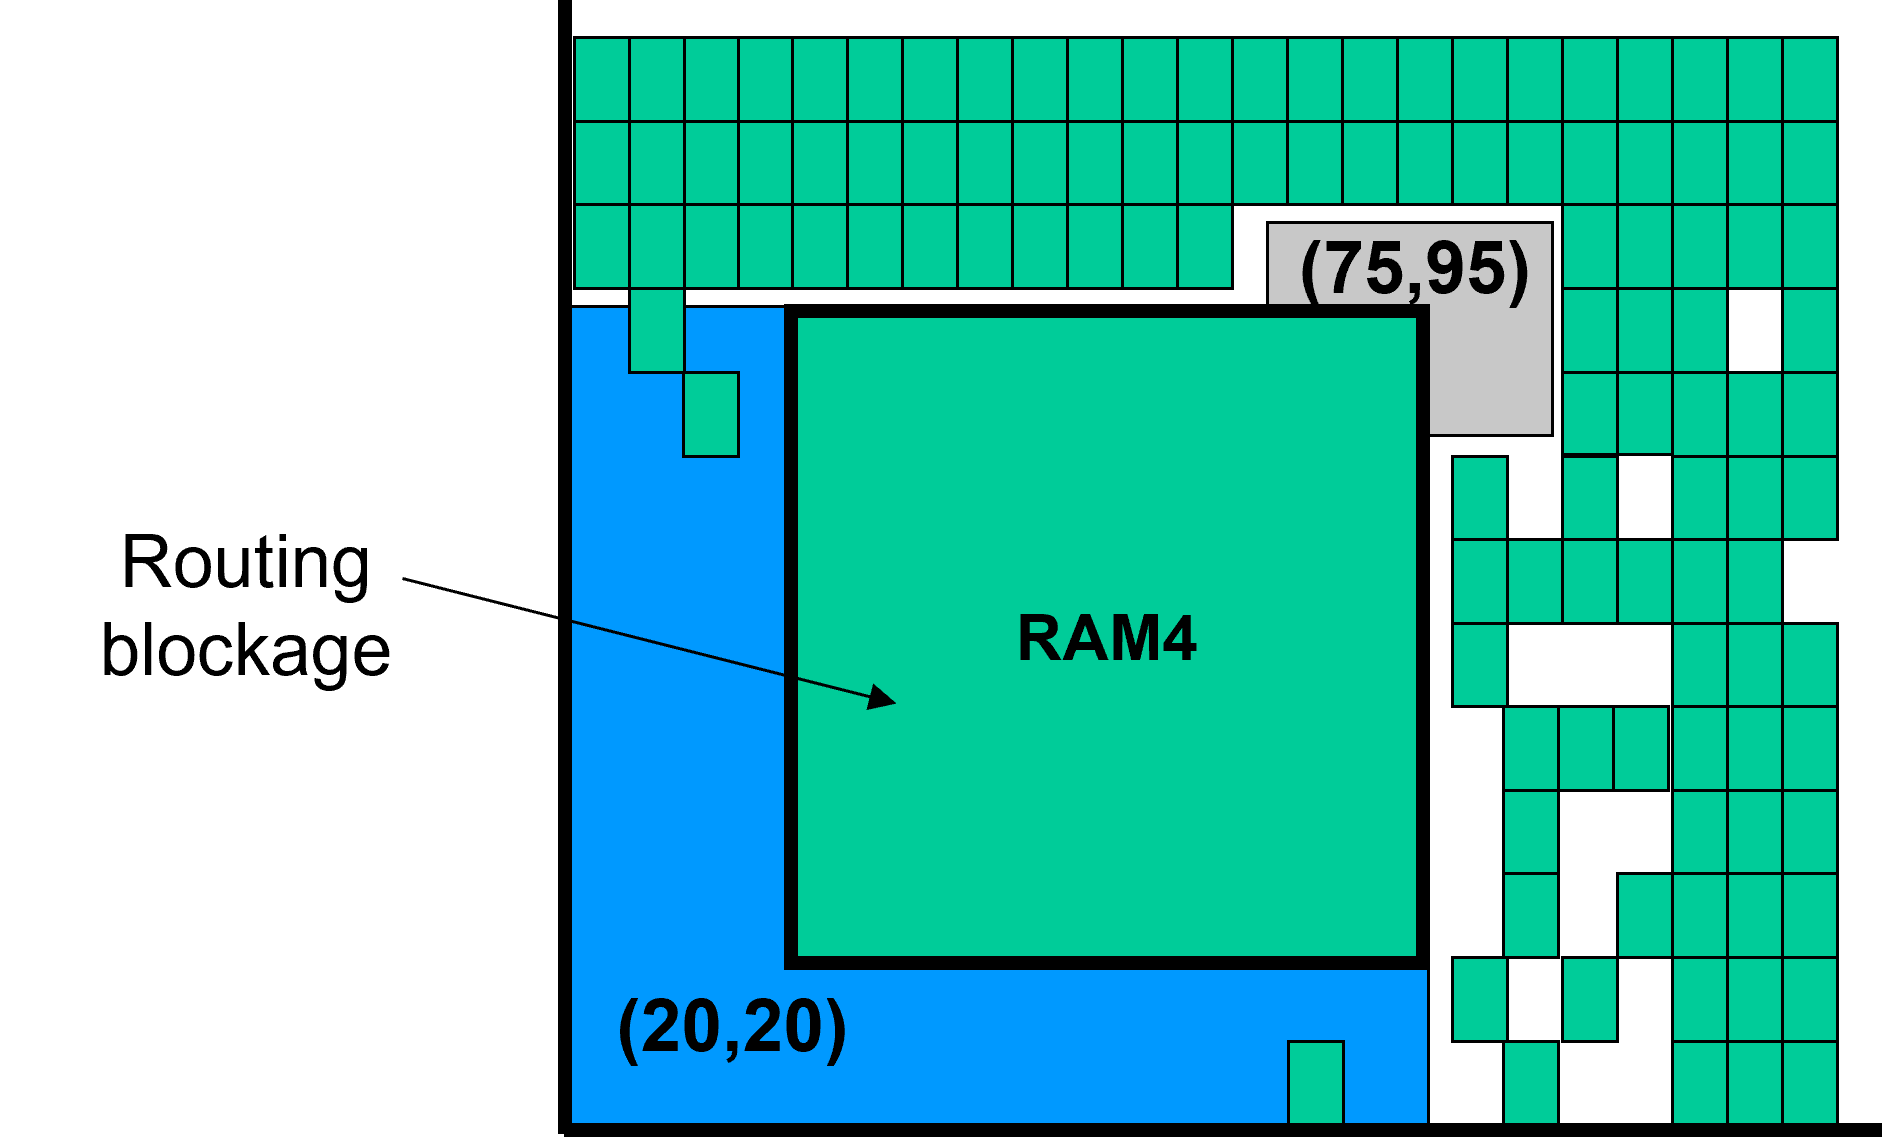
\includegraphics[width= \textwidth]{RoutingBlockage}
			\end{center}
		\end{columns}
\end{frame}
\begin{frame}
	\frametitle{Guidelines for a good floorplan}
	\begin{center}
		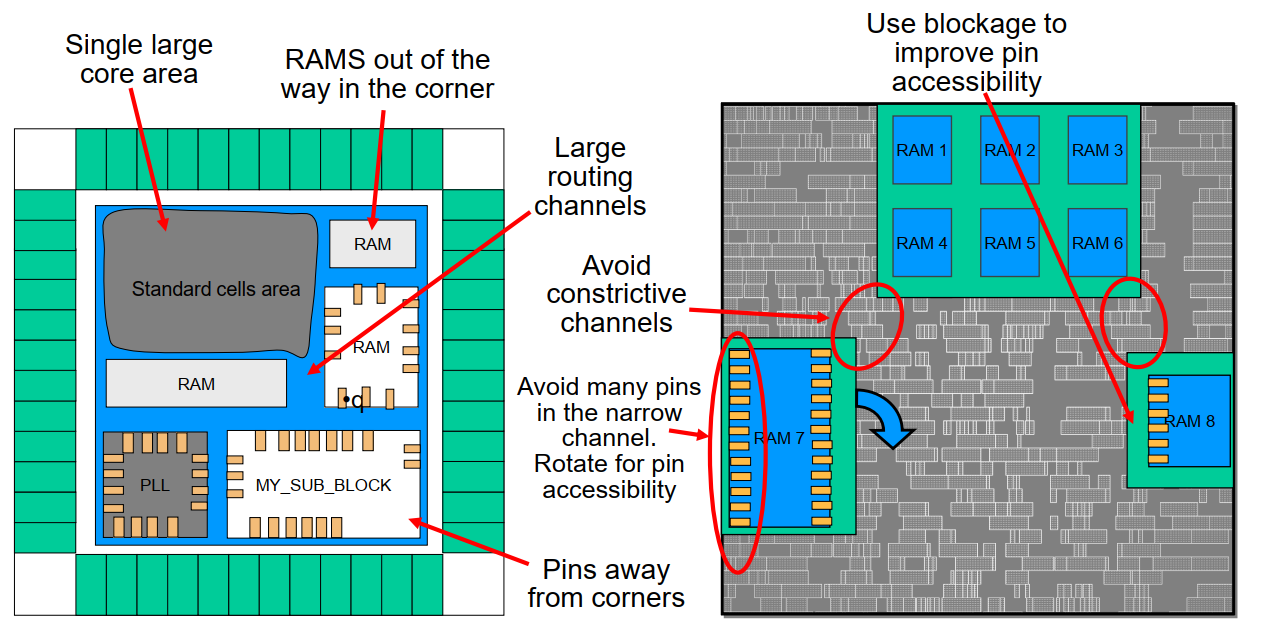
\includegraphics[width=\textwidth]{Macro3}
	\end{center}
\end{frame}

\subsection[PAD]{Pad Area}
\begin{frame}
	\frametitle{Pad Area}
	\begin{columns}	
		\column{0.6\textwidth}
		\begin{itemize}
			\item \textbf{Pad area consists of:}
				\begin{itemize}
					\item Input/Output/InOut pads
					\item Power pads and corner pads
					\item Pad fillers
					\item P/G rings
				\end{itemize}
		\end{itemize}
		\column{0.5\textwidth}
		\begin{center}
			\includegraphics[width=0.8\textwidth]{pad}
		\end{center}
	\end{columns}
\end{frame}
\begin{frame}
	\frametitle{Pin Alignment}
		\begin{itemize}
			\item Pin alignment is not less important than macros alignment. 
			\item In the case of macros, wire length is reduced, and the area is increased. In the case of Pin alignment, wire length is reduced, and the area remains the same
		\end{itemize}
		\begin{center}
			\includegraphics[width=0.7\textwidth]{pin}
		\end{center}
\end{frame}

\begin{frame}
	\frametitle{Hierarchical Approach}
		\begin{columns}	
		\column{0.6\textwidth}
		\begin{itemize}
			\item \textbf{Chip is partitioned into smaller blocks}
		\item \textbf{Each block is P\&R'ed
		individually }
		\item \textbf{Blocks are integrated
		back into the chip	}		
		\end{itemize}
		\column{0.6\textwidth}
		\begin{center}
			\includegraphics[width=0.7\textwidth]{partitioning}
		\end{center}
	\end{columns}
\end{frame}
\begin{Form}
	\frametitle{Chip vs. Block}
			\begin{columns}	
		\column{0.5\textwidth}
		\begin{itemize}
			\item \textbf{Chip has:}
				\begin{itemize}
					\item Pads (signal and P/G)
				\end{itemize}
			\item \textbf{Block has: }		
				\begin{itemize}
					\item Pins (signal and P/G)
				\end{itemize}
			
				\item \textbf{Blocks can be
				rectangular or
				rectilinear in shape.}
					
		\end{itemize}
		\column{0.6\textwidth}
		\begin{center}
			\includegraphics[width=0.7\textwidth]{partitioning}
		\end{center}
	\end{columns}
\end{Form}
	%--------------------------------------------------	
	\begin{frame}
		\frametitle{....}
		\begin{center}
			\<بِسْمِ اللَّـهِ الرَّحْمَـٰنِ الرَّحِيمِ> \\
			\<وَمَا أُوتِيتُمْ مِنَ الْعِلْمِ إِلَّا قَلِيلًا>
			
		\end{center}
	\end{frame}
	%---------------------------------------------	
\end{document}	